\section{高等数学}
\subsection{初等数学提挈}
\subsubsection{常用三角函数公式}
\begin{align*}
    \sin^2 \alpha + & \cos^2\alpha = 1 &
    \tan^2 \alpha + & 1 = \sec^2 \alpha \\
    \cot \alpha  & =\frac{1}{\tan \alpha} &
    \cot^2 \alpha + & 1 = \csc^2 \alpha \\
    \csc \alpha & =\frac{1}{\sin \alpha} &
    \sec \alpha & = \frac{1}{\cos \alpha} 
\end{align*}
\begin{enumerate}
\item 两角和差公式
\begin{gather*}
    \sin(\alpha+\beta)=\sin\alpha\cos\beta+\cos\alpha\sin\beta \\
    \sin(\alpha-\beta)=\sin\alpha\cos\beta-\cos\alpha\sin\beta \\
    \cos(\alpha+\beta)=\cos\alpha\cos\beta-\sin\alpha\sin\beta \\
    \cos(\alpha-\beta)=\cos\alpha\cos\beta+\sin\alpha\sin\beta\\
    \tan(\alpha+\beta)=\frac{\tan\alpha+\tan\beta}{1-\tan\alpha\tan\beta}\\
    \tan(\alpha-\beta)=\frac{\tan\alpha-\tan\beta}{1+\tan\alpha\tan\beta}
\end{gather*}
\item 积化和差公式
\begin{align*}
    \sin \alpha \cos \beta & =\frac{1}{2}[\sin (\alpha+\beta)+\sin(\alpha-\beta)]  \\
    \cos \alpha \sin \beta & =\frac{1}{2}[\sin (\alpha+\beta)-\sin(\alpha-\beta)]  \\
    \cos \alpha \cos \beta & =\frac{1}{2}[\cos (\alpha+\beta)+\cos(\alpha-\beta)]  \\
    \sin \alpha \sin \beta & =-\frac{1}{2}[\cos (\alpha+\beta)-\cos(\alpha-\beta)]
\end{align*}
\item 和差化积公式
\begin{align*}
    \sin\alpha+\sin\beta & =2\sin\frac{\alpha+\beta}{2}\cos\frac{\alpha-\beta}{2}  \\
    \sin\alpha-\sin\beta & =2\cos\frac{\alpha+\beta}{2}\sin\frac{\alpha-\beta}{2}  \\
    \cos\alpha+\cos\beta & =2\cos\frac{\alpha+\beta}{2}\cos\frac{\alpha-\beta}{2}  \\
    \cos\alpha-\cos\beta & =-2\sin\frac{\alpha+\beta}{2}\sin\frac{\alpha-\beta}{2} \\
    \tan\alpha+\tan\beta & =\frac{\sin (\alpha+\beta)}{\cos\alpha\cdot\cos \beta}
\end{align*}
\item 倍角公式
\begin{align*}
    \cos 2\alpha & =\cos^2 \alpha-\sin^2\alpha=2\cos^2\alpha-1=1-2\sin^2\alpha\\
    \sin 2\alpha  & =2\sin \alpha \cos \alpha\\
    \tan 2\alpha  & =\frac{2\tan\alpha}{1-\tan^2\alpha}, \tan\alpha=\frac{\sin2\alpha}{1+\cos2\alpha}=\frac{1-\cos2\alpha}{\sin2\alpha}
\end{align*}
\end{enumerate}

\subsubsection{排列组合}
$A_n^m$表示从$n$个不同的元素中取出$m$个元素的排列;

$C_n^m$表示从$n$个不同的元素中取出$m$个元素的组合.
\begin{align*}
    0!&=1 & 
    n!&=n\cdot (n-1)\cdot (n-2) \dots 2\cdot 1\\
    A_n^m&=\frac{n!}{(n-m)!} & 
    C_n^m&=\frac{n!}{m!\times (n-m)!}\\
\end{align*} 
二项式定理:
\begin{align*}
    (a+b)^n&=\sum^{n}_{k=0}\mathbf{C} _n^ka^{n-k}b^k \\
    &=a^n+na^{n-1}b+\frac{n(n-1)}{2!}a^{n-2}b^2\\
    &+\dots+\frac{n(n-1)\dots(n-k+1)}{k!}a^{n-k}b^k+\dots+nab^{n-1}+b^n.
\end{align*}

因式分解:
\begin{align*}
    a^3+b^3=(a+b)(a^2-ab+b^2)\\
    a^3-b^3=(a-b)(a^2+ab+b^2)\\
\end{align*}

\subsubsection{常见的几种初等函数图像及其性质}

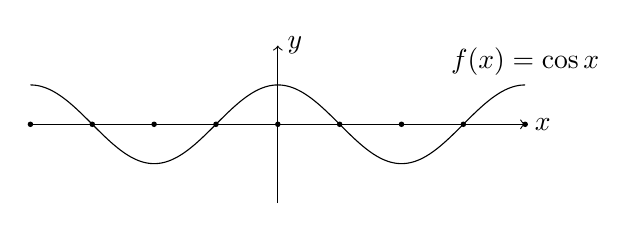
\begin{tikzpicture}[scale=0.5,smooth,samples=100]
    \draw[->](-2*pi,0) -- (2*pi,0) node[right] {$x$};
    \draw[->](0,-2) -- (0,2) node[right] {$y$};
    \foreach \x in {-2,-3/2,-1,-0.5,0,0.5,1,1.5,2}
        {\fill (\x*pi,0) circle (2pt);
        }
    \draw [domain=-2*pi:2*pi] plot (\x,{cos(\x r)}) node[above] {$f(x) = \cos x$};
\end{tikzpicture}
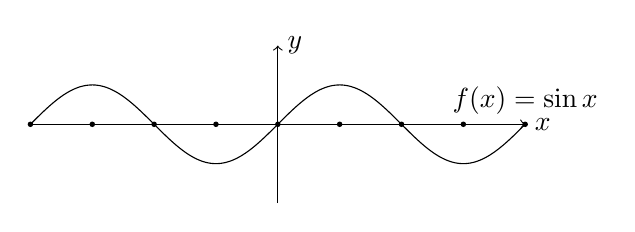
\begin{tikzpicture}[scale=0.5,smooth,samples=100]
    \draw[->](-2*pi,0) -- (2*pi,0) node[right] {$x$};
    \draw[->](0,-2) -- (0,2) node[right] {$y$};
    \foreach \x in {-2,-3/2,-1,-0.5,0,0.5,1,1.5,2}
        {\fill (\x*pi,0) circle (2pt);
        }
    \draw [domain=-2*pi:2*pi] plot (\x,{sin(\x r)}) node[above] {$f(x) = \sin x$};
\end{tikzpicture}

\begin{tikzpicture}[scale=0.5,smooth,samples=100]
    \draw[->](-2*pi,0) -- (2*pi,0) node[right] {$x$};
    \draw[->](0,-5) -- (0,5) node[right] {$y$};
    \foreach \x in {-2,-3/2,-1,-0.5,0,0.5,1,1.5,2}
        {\fill (\x*pi,0) circle (2pt);
        }
    \draw [domain=-2*pi+0.2:-pi-0.2] plot (\x,{cot(\x r)});
    \draw [domain=-pi+0.2:-0.2] plot (\x,{cot(\x r)});
    \draw [domain=0.2:pi-0.2] plot (\x,{cot(\x r)});
    \draw [domain=pi+0.2:2*pi-0.2] plot (\x,{cot(\x r)}) node[below] {$f(x) = \cot x$};
\end{tikzpicture}
\begin{tikzpicture}[scale=0.5,smooth,samples=100]
    \draw[->](-2*pi,0) -- (2*pi,0) node[right] {$x$};
    \draw[->](0,-5) -- (0,5) node[right] {$y$};
    \foreach \x in {-2,-3/2,-1,-0.5,0,0.5,1,1.5,2}
        {\fill (\x*pi,0) circle (2pt);
        }
    \draw [domain=-2*pi+0.2:-pi-0.2] plot (\x,{1/sin(\x r)});
    \draw [domain=-pi+0.2:-0.2] plot (\x,{1/sin(\x r)});
    \draw [domain=0.2:pi-0.2] plot (\x,{1/sin(\x r)});
    \draw [domain=pi+0.2:2*pi-0.2] plot (\x,{1/sin(\x r)}) node[below] {$f(x) = \csc x$};
\end{tikzpicture}

\begin{tikzpicture}[scale=0.5,smooth,samples=100]
    \draw[->](-2*pi,0) -- (2*pi,0) node[right] {$x$};
    \draw[->](0,-5) -- (0,5) node[right] {$y$};
    \foreach \x in {-2,-3/2,-1,-0.5,0,0.5,1,1.5,2}
        {\fill (\x*pi,0) circle (2pt);
        }
    \draw [domain=-2*pi:-1.5*pi-0.2] plot (\x,{1/cos(\x r)});
    \draw [domain=-1.5*pi+0.2:-0.5*pi-0.2] plot (\x,{1/cos(\x r)});
    \draw [domain=-0.5*pi+0.2:0.5*pi-0.2] plot (\x,{1/cos(\x r)});
    \draw [domain=0.5*pi+0.2:1.5*pi-0.2] plot (\x,{1/cos(\x r)});
    \draw [domain=1.5*pi+0.2:2*pi] plot (\x,{1/cos(\x r)}) node[right] {$f(x) = \sec x$};
\end{tikzpicture}
\begin{tikzpicture}[scale=0.5,smooth,samples=100]
    \draw[->](-5,0) -- (5,0) node[right] {$x$};
    \draw[->](0,-3) -- (0,3) node[right] {$y$};
    \draw [domain=-5:5] plot (\x,{ln(\x+sqrt(1+\x*\x))}) node[above] {$f(x)=\ln(x+\sqrt{1+x^2})$};
\end{tikzpicture}

\subsubsection{解方程}
\begin{examp}{$
    \begin{dcases}
        \sin x_0+a\cos x_0=a+\frac{1}{2}\\
        \tan x_0 =\frac{1}{a}.
    \end{dcases}$其中$a$为常数,求$a$.}
    
    \jie 将二式代入一式消去$\sin x$,化简后画三角形解方程:
    \begin{gather*}
        \begin{dcases}
            \cos x_0=\frac{a^2+\frac{1}{2}a}{a^2+1},\\
            \tan x_0 =\frac{1}{a}.
        \end{dcases}
        \hfill
        \begin{tikzpicture}[baseline=(char.base)]
            \node(char) at (0,0) {};
            \draw(0.5,-0.8) coordinate (A)--(3.5,-0.8) coordinate (B)--(3.5,0.8) coordinate (C)--cycle pic ["$x_0$",draw,angle radius=0.5cm,angle eccentricity=2] {angle = B--A--C};
            \node (cha) at ($(0.5,-1)!0.5!(3.5,-1)$) [below] {$a$};
            \node (cha) at ($(3.5,-0.8)!0.5!(3.5,0.8)$) [right] {$1$};
            \node (cha) at ($(0.5,-1)!0.5!(3.5,0.8)$) [above,xshift=-1cm] {$\sqrt{a^2+1}$};
        \end{tikzpicture}\\
        \implies \cos x_0=\frac{a}{\sqrt{a^2+1}}=\frac{a^2+\frac{1}{2}a}{a^2+1}
        \implies a=\frac{3}{4}
    \end{gather*}
\end{examp}

\subsubsection{不等式}
\begin{figure}[htp]
\centering
\begin{tikzpicture}
    \matrix 
    {
    \node(a1){调和平均值}; & & \node(a2){几何平均值}; & & \node(a3){算术平均值}; & & \node(a4){平方平均值}; \\
    \node(b1){$\dfrac{2}{\dfrac{1}{x}+\dfrac{1}{y}}$}; & \node{$\leqslant$}; & \node(b2){$\sqrt{xy} $}; & \node{$\leqslant$}; & \node(b3){$\dfrac{x+y}{2} $}; & \node{$\leqslant$}; & \node(b4){$\sqrt{\dfrac{x^2+y^2}{2}}$}; \\
    };
\end{tikzpicture}
\end{figure}
一个更一般的结论:
\begin{align*}
    \frac{n}{\sum\limits^{n}_{i=1}\frac{1}{a_i}}\leqslant \sqrt[n]{\prod^n_{i=1}a_i} \leqslant\frac{\sum\limits^{n}_{i=1}a_i}{n} \leqslant \sqrt{\frac{\sum\limits^{n}_{i=1}a_i^2}{n}}
\end{align*}

与绝对值有关的不等式:
\begin{align*}
    \left\lvert a\pm b\right\rvert \leqslant & \left\lvert a\right\rvert +\left\lvert b\right\rvert .&
    \left\lvert \left\lvert a\right\rvert -\left\lvert b\right\rvert \right\rvert \leqslant & \left\lvert a-b\right\rvert. \\
    \left\lvert a_1\pm a_2\pm \dots\pm a_n\right\rvert  \leqslant & \left\lvert a_1\right\rvert +\left\lvert a_2\right\rvert + \dots \left\lvert a_n\right\rvert. &
    \left\lvert \int_{b}^{a} f(x) \,\mathrm{d}x \right\rvert \leqslant & \int_{b}^{a} \left\lvert f(x)\right\rvert  \,\mathrm{d}x.\\
    \frac{1}{x+1}<\ln \left(1+\frac1x \right) < & \frac{1}{x} ,(x>0). &
    \left\lvert ab\right\rvert \leqslant & \frac{a^2+b^2}{2}.
\end{align*}
\begin{prf}
    \begin{gather*}
        \sqrt{ab} \leqslant\frac{a+b}{2}\implies \sqrt{a^2b^2} =\left\lvert ab\right\rvert \leqslant\frac{a^2+b^2}{2}
    \end{gather*}
\end{prf}
证明不等式的问题有两种思路,一种是把问题转化为函数$f(x)$在定义域内恒大于或小于0;另一种是比较不等式两边的函数在定义域内的最大值和最小值的问题,适用于不等式两边过于复杂的情况
\begin{examp}{证明:$\left(\ln \frac{1+x}{x}-\frac{1}{1+x}\right) ^2<\frac{1}{x(1+x)^2},(x>0).$}
\end{examp}

证明两个变量的不等式的思路是要么把两个变量化成一个,要么把其中一个变量当作常数化为恒成立问题,这是通用的方法.但合适的时候使用拉格朗日中值定理大大方便了证明.

\begin{examp}{设$0<a<b,$证明:$\ln \frac{b}{a}>2\frac{b-a}{a+b}.$}
    \par \jie 把不等式右边化为$\frac{\frac{b}{a}-1}{\frac{b}{a}+1}.$
\end{examp}
证明积分不等式有一个常用的方法,构造积分变限函数,可令:
\begin{equation*}
    (a-b)f(x)=\int_{a}^{b} f(x) \,\mathrm{d}t \text{或} f(x)\int_{a}^{b}  \,\mathrm{d}t .
\end{equation*}
\begin{examp}{设$f(x)$在$[a,b]$上连续,且$f(x)>0$.证明:$\int_{a}^{b} f(x) \,\mathrm{d}x \cdot \int_{a}^{b} \frac{1}{f(x)} \,\mathrm{d}x \geqslant (b-a)^2.$}
    \par \zheng 令$F(x)=\int_{a}^{x} f(t) \,\mathrm{d}t \cdot \int_{a}^{x} \frac{1}{f(t)} \,\mathrm{d}t -(x-a)^2, 0 \leqslant x \leqslant b. \\
    F'(x)=f(x)\int_{a}^{x} f(t) \,\mathrm{d}t +\int_{a}^{x} \frac{1}{f(t)} \,\mathrm{d}t \cdot \frac{1}{f(x)} =\int_{a}^{x} \left( \frac{f(x)}{f(t)}+\frac{f(t)}{f(x)}-2 \right) \,\mathrm{d}t \geqslant 0,\\
    F(x)$单调递增,故$F(b)> F(a)=0$.
\end{examp}
\begin{examp}{设$f(x)$在$[0,1]$上连续,且单调递减.证明:当$0<\lambda<1$时,$\int_{0}^{\lambda} f(x) \,\mathrm{d}x \geqslant \lambda \int_{0}^{1} f(x) \,\mathrm{d}x .$}
    \par \zheng 观察到右边$\int_{0}^{1} f(x) \,\mathrm{d}x $是一个常数,故把$\lambda$移到左边.要证$\int_{0}^{\lambda} f(x) \,\mathrm{d}x \geqslant \lambda \int_{0}^{1} f(x) \,\mathrm{d}x $,只要证$\frac{\int_{0}^{\lambda} f(x) \,\mathrm{d}x }{\lambda}\geqslant \int_{0}^{1} f(x) \,\mathrm{d}x $,令$F(\lambda)=\frac{\int_{0}^{\lambda} f(x) \,\mathrm{d}x }{\lambda},\\ 
    F'(\lambda)=\frac{f(\lambda)\cdot \lambda-\int_{0}^{\lambda} f(x) \,\mathrm{d}x }{\lambda^2}=\frac{f(\lambda)\int_{0}^{\lambda}  \,\mathrm{d}x -\int_{0}^{\lambda} f(x) \,\mathrm{d}x }{\lambda^2}=\frac{\int_{0}^{\lambda} [f(\lambda)-f(x)] \,\mathrm{d}x }{\lambda^2}<0,\\
    F(\lambda)$单调递减,故$F(\lambda) > F(1) = \int_{0}^{1} f(x) \,\mathrm{d}x $,即$\int_{0}^{\lambda} f(x) \,\mathrm{d}x \geqslant \lambda \int_{0}^{1} f(x) \,\mathrm{d}x .$
\end{examp}
\begin{examp}{设$0<a<b<1,$证明:$\arctan b-\arctan a<\frac{b-a}{2ab}.$}
    \par \zheng 构造$f(x)=\arctan x.$由拉格朗日中值定理,存在$\xi \in (a,b),f'(\xi)=\frac{f(b)-f(a)}{b-a}\implies \frac{1}{1+\xi^2}=\frac{\arctan b-\arctan a}{b-a},\frac{1}{1+\xi^2}<\frac{1}{1+a^2}<\frac{1}{b^2+a^2}<\frac{1}{2ab}\implies \arctan b-\arctan a<\frac{b-a}{2ab}.$
\end{examp}

\subsection{极限}
\subsubsection{求取极限的几种重要方法}
\begin{enumerate}
    \item 两个重要的极限:
\begin{align*}
    \lim_{x \to 0}\frac{\sin x}{x}=1,\\
    \lim_{x \to \infty}\left(1+\frac{1}{x}\right)^x=\mathrm{e}.
\end{align*}

由第二个重要极限可以推出,若$\lim u^v$属于$1^\infty$型,那么
\begin{equation*}
    \lim u^v=\mathrm{e}^{\lim (u-1)v}.
\end{equation*}

\begin{prf}
    \begin{gather*}
        \lim u^v=\lim \left[(u-1+1)^{\frac{1}{u-1}}\right]^{(u+1)v}=\mathrm{e}^{\lim (u-1)v}
    \end{gather*}
\end{prf}

\item 等价无穷小量替换

当$x\to 0$时,几个重要的等价无穷小量替换:
\begin{align*}
    \sin x &\sim x & \tan x &\sim x\\
    \arcsin x &\sim x & \arctan x &\sim x\\
    \ln(1+x) &\sim x & e^x-1 &\sim x\\
    a^x-1 &\sim x\ln a & 1-\cos x &\sim \frac{1}{2}x^2\\
    (1+x)^\alpha-1 &\sim \alpha x & (1+x)^\alpha-1 &\sim \alpha x
\end{align*}

当$x \to x_0 $时,若$f(x) \to 0, g(x) \to 0,$则有$\mathrm{e}^{f(x)}-\mathrm{e}^{g(x)}\sim f(x)-g(x).$

\txe{注:$\mathrm{e}^{\tan x}-\mathrm{e}^{x}\sim \tan x-x.$}

\zheng $\mathrm{e}^{f(x)}-\mathrm{e}^{g(x)}=\mathrm{e}^{f(x)}(1-\mathrm{e}^{g(x)-f(x)})\sim -\mathrm{e}^{f(x)}(g(x)-f(x))\sim f(x)-g(x).$\hfill$\blacksquare $

当$f(x) \to 0,g(x) \to 1 $时,若出现$\mathrm{e}^{f(x)}$或$\ln g(x)$,则要考虑进行凑配,将上述式子变成$\mathrm{e}^{f(x)}-1+1$和$\ln [g(x)-1+1]$,由于$x\to 0,\mathrm{e}^x-1\sim x, \ln (x+1)\sim x$,所以$\mathrm{e}^{f(x)}-1+1\sim f(x)+1,\ln [g(x)-1+1]\sim g(x)-1$.

当$f(x)\to 0$,对$a^{f(x)}-1$,都化作$\mathrm{e} ^{{f(x)}\ln a}-1,$.
\begin{examp}
    $2^x-1=\mathrm{e} ^{\ln 2^x}-1=\mathrm{e} ^{x\ln 2}-1=x\ln 2,x\to 0$.
\end{examp}

\begin{ttheorem}
    有界函数和无穷小量的乘积仍为无穷小量.
\end{ttheorem}

\begin{examp}{$\lim_{x \to 0} x^2\cdot\sin \frac{1}{x}=0$}
    
\end{examp}

\begin{examp}{$\lim_{x \to \infty} \frac{2x^2-3}{5x^2+2\sin x}$}

    \jie 构造无穷小量解决$\sin x$.
    
    $\lim_{x \to \infty} \frac{2x^2-3}{5x^2+2\sin x}=\lim_{x \to \infty} \frac{2-\frac{3}{x^2}}{5+\frac{2}{x^2}\sin x}=\frac{2}{5}.$
\end{examp}

\item 泰勒展开

当$x\to 0$时,几个重要的泰勒展开式:
\begin{align*}
    \arcsin x &= x +\frac{x^3}{3!}+o(x^3) & \arctan x &= x -\frac{x^3}{3}+o(x^3)\\
    \tan x &=x+\frac{x^3}{3}+o(x^3) & &
\end{align*}
\txe{注:记忆技巧:tan分母无阶乘,反三角函数符号异,sin与tan符号异.}

使用泰勒公式求极限时,要注意高阶无穷小量是否趋向于0.
\begin{examp}
    {$\lim_{n \to \infty} \frac{\mathrm{e} ^{\frac{1}{n^2}}-\cos \frac{\pi}{n}}{\frac{1}{n^2}},n \to \infty,o(\frac{1}{n}) \to 0.$}
\end{examp}

\begin{examp}
    {$\lim_{n \to \infty} a\cdot \left( \frac{n}{n+1} \right)^n=\lim_{n \to \infty} a\cdot \left( \frac{1}{1+\frac{1}{n}} \right)^n=\lim_{n \to \infty} a\cdot  \frac{1}{\left(1+\frac{1}{n}\right) ^n} =\frac{a}{\mathrm{e} }.$}
\end{examp}

无穷小量的运算规则:
\begin{gather*}
    o(x^m)+o(x^n)=o(x^l),l=\min\left\{m,n\right\} \\
    o(x^m)\cdot o(x^n)=o(x^{m+n}),x^m\cdot o(x^n)=o(x^{m+n})\\
    k\cdot o(x^m)=o(x^m)
\end{gather*}

\item 几个定式:

对于形如$a^x+b^x$式子的处理方法:提取$a^x\left[1+\left(\frac{b}{a}\right) ^x\right] $;

对于形如$a^x+a^y$式子的处理方法:提取$a^x \left(1+a^{y-x} \right)$;

对于形如$a^x+b^y$式子的处理方法:提取$a^x \left(1+\frac{b^y}{a^x} \right)$ .

若$\left\lvert q\right\rvert <1,\lim_{n \to \infty}q^n=0$.

\item 拉格朗日中值定理:


\item 洛必达法则

出现$0/0,\infty/\infty$型的极限采用洛必达法则进行计算,在洛的过程中适当加入等价无穷小量代换可以降低计算难度.

\enumlabel{1.}对于$\infty\pm\infty$型要先观察能否通分化简转换成第一种情况,如果不可以,再观察有无形如$1/x$的变量,然后换元转换成第一种情况;如果既不能通分也不能换元就考虑把所有式子对数化,让后用对数运算法则变为两个数相乘.
\begin{examp}
    {$\lim_{x \to \infty}\left[\ln (\mathrm{e}^x+1)-x \right] = \lim_{x \to \infty}\left[\ln (\mathrm{e}^x+1)+\ln \mathrm{e}^{-x} \right] \\= \lim_{x \to \infty}\ln (\mathrm{e}^x+1)\mathrm{e}^{-x}=0.$}
\end{examp}
\begin{examp}
    {$\lim_{x \to +\infty}(\ln x-\frac{x}{\mathrm{e}}+k)=\lim_{x \to +\infty}(\ln x-\ln e^{x/\mathrm{e}}+k)=\ln \lim_{x \to +\infty}\frac{x}{e^{x/e}}+k=\ln \lim_{x \to +\infty}\frac{e}{e^{x/e}}+k=-\infty+k=-\infty$}
\end{examp}

\enumlabel{2.}对于$0^\infty,\infty^\infty$则将原式化为$\mathrm{e}$的指数再求极限:$u^v=e^{\ln u^v}=e^{v\ln u}.$使用洛必达法则遇到$e^{-x}$要将它放到分母上.
\begin{examp}
    {$\lim_{x \to \infty}x^2e^{-2x}=\lim_{x \to \infty}\frac{x^2}{e^{2x}},\lim_{x \to -\infty}xe^x=\lim_{x \to -\infty}\frac{x}{1/e^x}$.}
\end{examp}

\begin{examp}
    {$\lim_{x \to 0} x^x=1$}
\end{examp}

\begin{examp}{$\lim_{x \to 1^{-}} \frac{1}{x-1}\mathrm{e} ^{\frac{1}{x^2-1}}$}

    \jie 注意$(1^-)^2-1<0,(1^-)^2=1^-$,
    
    $\lim_{x \to 1^{-}} \frac{1}{x-1}\mathrm{e} ^{\frac{1}{x^2-1}}=\lim_{x \to 1^{-}} -\frac{2x}{(x^2-1)^2}\mathrm{e} ^{\frac{1}{x^2-1}}\\
    =\lim_{x \to 1^{-}} 2x\cdot\lim_{x \to 1^{-}} -\frac{1}{(x^2-1)^2}\mathrm{e} ^{\frac{1}{x^2-1}}$,换元,令$t=\frac{1}{x^2-1}$,得$-2 \lim_{t \to -\infty} t^2 \mathrm{e} ^t=-2 \lim_{t \to -\infty} \frac{t^2}{\frac{1}{\mathrm{e} ^t}}=-2 \lim_{t \to -\infty} \frac{2t}{-\frac{1}{\mathrm{e} ^t}}=-2 \lim_{t \to -\infty} \frac{2}{\frac{1}{\mathrm{e} ^t}}=-2 \lim_{t \to -\infty} 2 \mathrm{e} ^t=0$
\end{examp}

\end{enumerate}

\subsubsection{极限的运算法则}
\begin{enumerate}
    \item $\lim \left[k f(x) \pm l g(x)\right] =k\lim f(x)+l\lim g(x)$.
    \item $\lim \left[f(x)\cdot g(x)\right] =\lim f(x)\cdot \lim g(x)$.
\end{enumerate}

形如$\displaystyle \lim_{x \to x_0} \frac{f(x)-g(x)}{h(x)}$的极限:
\begin{enumerate}
    \item 求分数的极限要注意是否是无穷小量比阶,若是无穷小量比阶,当式子中出现加减运算,求极限时不能采用等价无穷小量替换,可以用泰勒展开,也可以用洛必达法则.这是因为等价无穷小量替换的精度太低,往往只展开到一阶,这往往比分母的阶数小,我们可以写出它的高阶无穷小量$o(x)$来比较其与分母的阶数.
    
    \item 若$\lim_{x \to x_0} g(x)=0$,可以用极限的四则运算法则将式子拆成
    \begin{equation*}
        \lim_{x \to x_0} \left(\frac{f(x)}{h(x)}-\frac{g(x)}{h(x)}\right) ,
    \end{equation*}
    分别求极限.注意!这里不能直接认为$\lim_{x \to x_0} \frac{f(x)-g(x)}{h(x)}=\lim_{x \to x_0} \frac{f(x)-0}{h(x)}$,因为当$\lim_{x \to x_0} h(x)=0$时,$\lim_{x \to x_0} \frac{g(x)}{h(x)}$分子分母都为0,此时是无穷小量比阶,可以使用洛必达法则和泰勒展开,但不能用等价无穷小量替换!直接将$g(x)=0$代入原式很容易忽略这一点!所以一定要拆分后再分别求极限.

    \item 对于$\displaystyle \lim_{h \to 0} \frac{\frac{f(x_0+h)-f(x_0)}{h}-f'(x_0)}{h}$不能当作$\displaystyle \lim_{h \to 0} \frac{f'(x_0)-f'(x_0)}{h}$,这是因为如果将这个极限拆开$\lim_{h \to 0} \frac{f(x_0+h)-f(x_0)}{h^2}\neq f'(x_0)$,分子分母的阶数不同,不符合导数的定义.
\end{enumerate}

\subsubsection{计算处理技巧}
对式子凑配后换元.

当$\lim_{x \to -\infty}$时,要注意$x$取值的正负是否会对极限产生影响,尤其在需要把$x$放进根号里时,$x<0$,放进根号时根号前要加负号.$x=-\left\lvert x\right\rvert =-\sqrt{x^2},x<0$.
\begin{equation*}
    f(x)=\frac{\sqrt{x^2+1}}{x}=
    \begin{dcases}
        \sqrt{\frac{x^2+1}{x^2}},x>0\\
        -\sqrt{\frac{x^2+1}{x^2}},x<0
    \end{dcases}
    \text{或}
    \lim_{x \to a}\frac{\ln (1+\mathrm{e}^{2x})}{\ln (1+\mathrm{e}^x)}=
    \begin{dcases}
        2,a=+\infty\\
        0,a=-\infty
    \end{dcases}
\end{equation*}
同理的还有如
\begin{equation*}
    \lim_{x \to a^+} \frac{\left\lvert f(x)\right\rvert }{x-a}=\lim_{x \to a^+} \left\lvert \frac{f(x)}{x-a}\right\rvert ,\lim_{x \to a^-} \frac{\left\lvert f(x)\right\rvert }{x-a}=-\lim_{x \to a^-} \left\lvert \frac{f(x)}{x-a}\right\rvert 
\end{equation*}

\begin{examp}{$I=\lim_{x \to -\infty} \frac{\sqrt{4x^2+x-1}+x+1}{\sqrt{x^2+\sin x}}$}

    \jie $I=\lim_{x \to -\infty} \frac{3x^2-x-2}{\sqrt{x^2+\sin x}(\sqrt{4x^2+x-1}-x-1)}\\
    =\lim_{x \to -\infty} \frac{3-\frac{1}{x}-\frac{2}{x^2}}{-\sqrt{1+\frac{\sin x}{x^2}}\left(-\sqrt{4+\frac{1}{x}-\frac{1}{x^2}}-1-\frac{1}{x}\right) }=1$,本题也可以分子分母直接同除$x$.
\end{examp}

\subsubsection{极限的性质}
若函数的极限存在,那么我们可以利用极限的性质得到一些关键的信息.\enumlabel{1.}无穷小量比阶:若有$x \to a,g(x) \to 0,\lim_{x \to a}\frac{f(x)}{g(x)}=c,c$是常数,说明$f(x),g(x)$是同阶无穷小量,即$\lim_{x \to a}f(x)=0.$ 比较常见的是$\lim_{x \to 0}\frac{f(x)}{x}=1.$若有$x \to a,g(x) \to 0,\lim_{x \to a}\frac{f(x)}{g(x)}=0,$说明$f(x)$是比$g(x)$高阶的无穷小量. 

\enumlabel{2.}极限的唯一性:若有$\lim_{x \to a}f(x)$存在,那么$\lim_{x \to a^-}f(x)=\lim_{x \to a^+}f(x)=\lim_{x \to a}f(x).$ 

\enumlabel{3.}极限的局部保号性:构造函数$F(x)=\frac{f(x)}{g(x)},$若$\lim_{x \to x_0}F(x)>0,$那么在点$x_0$的邻域$(x_0-\delta,x_0+\delta)$内,始终有$F(x)>0,$若$g(x)>0,$那么就有$f(x)>0.$需要注意的是,如果函数极限在左(右)邻域取得,那么局部保号性也就是针对左(右)邻域而言的.若$\lim_{x \to x_0^+}F(x)>0,$那么在点$x_0$的右邻域$(x_0,x_0+\delta)$内,始终有$F(x)>0$.

无穷小量比阶的几种含义:当$\lim_{x \to x_0} f(x)=0,\lim_{x \to x_0} g(x)=0$时
\begin{enumerate}
    \item $f(x)$是$g(x)$的同阶无穷小量$\lim_{x \to x_0} \frac{f(x)}{g(x)}=A$,$A$为常数.
    \item $f(x)$是$g(x)$的等价无穷小量$\lim_{x \to x_0} \frac{f(x)}{g(x)}=1$
    \item $f(x)$是$g(x)$的高阶无穷小量$\lim_{x \to x_0} \frac{f(x)}{g(x)}=0$
    \item $f(x)$是$g(x)$的$n$阶无穷小量$\lim_{x \to x_0} \frac{f(x)}{(g(x))^n}=A$,$A$为常数.
    \item $f(x)$是$k$阶无穷小的含义,$\lim _{x \to x_0}\frac{f(x)}{x^k}=A$,$A$为常数.
\end{enumerate}

若$\lim _{x \to x_0}\frac{f(x)}{g(x)}=A$,$A$为常数,那么当$x \to x_0$时,$f(x)=Ag(x)$.

若我们得到了函数上某点的导数值$f'(x_0)>0$,我们就得出了在点$x_0$的邻域$(x_0-\delta,x_0+\delta)$内函数$f(x)$单调递增.若$f'(x)>0$,可得$n \to \infty,f(\frac{1}{n})>f(\frac{1}{n+1})$.

\subsubsection{函数的性质(极值、拐点、凹凸性)}
求函数的单调区间要画表.拐点是一个坐标,极值点是一个$x$的值.

$x_0$是函数$f(x)$的极值点的充分条件是
$\begin{dcases}
    f'(x_0)=0,\\
    f''(x_0)\neq 0.
\end{dcases}$
若$f''(x_0)>0$,那么函数取极小值点,若$f''(x_0)<0$,那么函数取极大值点.

如果$f''(x_0)=0$,函数$f(x)$也可以取到极值.如果函数$f(x)$在$x_0$的左邻域内$f'(x)>0$,右邻域内$f'(x)<0$,那么函数取到极大值,相反取到极小值.这时候就要判断$f''(x_0)$的邻域内的正负情况,要想取到极值,我们总是希望$f'(x)$是单调的,也就是$f''(x_0)$在邻域内符号总是保持不变.

$x_0$是函数$f(x)$的拐点的充分条件是
$\begin{dcases}
    f''(x_0)=0,\\
    f'''(x_0)\neq 0.
\end{dcases}$;

或者是当$f'''(x_0)=0$时,$f'''(x_0)$在邻域内符号总是保持不变.因为这样,函数$f(x)$在$x_0$的左右邻域内$f''(x_0)$的符号相反.

判断一个函数的凹凸性只要在他的图像上的某个区间内画一条割线,观察曲线对这条割线而言是凸的还是凹的.如果要判断函数在$x_0$附近的凹凸性,就看这个函数的二阶导数.凹函数的充要条件是$f''(x_0)>0,$凸函数的充要条件是$f''(x_0)<0.$值得注意的是,在极小值点附近函数是凹函数;在极大值点附近函数是凸函数,所以他们对应的二阶导条件是一致的.

判断函数的铅垂渐近线只要关注几个不在函数定义域内的点;判断水平渐近线和斜渐近线要关注函数在定义域内$x \to +\infty,x \to -\infty$时的情况;若$\lim_{x \to \infty} \frac{f(x)}{x}=a,\lim_{x \to \infty} \left[f(x)-ax\right] =b$,则$y=ax+b$是曲线$y=f(x)$的一条斜渐近线.若$\lim_{x \to \infty} f(x)=y_0$,则$y=y_0$是函数$y=f(x)$一条水平渐近线.

若函数$f(x)$有界,那么他一定有水平渐近线,同时斜渐近线的斜率应为0,即
\begin{equation*}
    \begin{dcases}
        \lim_{x \to \infty} f(x)=A,A\text{为常数}\\
        \lim_{x \to \infty} \frac{f(x)}{x}= 0 \implies \lim_{x \to \infty} f'(x)=0.
    \end{dcases}
\end{equation*}

\begin{theorem}[连续有界定理]
    若函数$f(x)$在$[a,b]$内连续,那么函数在$[a,b]$内有界.
\end{theorem}
如果函数在开区间$(a,b)$内连续,只要证明在端点处函数的极限存在,就能说明函数在$(a,b)$内有界.要想说明函数在$[a,b]$内连续,还要说明函数在端点处的极限值与端点处函数的定义相同.也就是说,若端点的极限值存在且和定义不同时,一个函数在$[a,b]$内不连续也可以是有界函数.

\subsection{导数与微分}
若函数$f(x)$在$x_0$处可导,则:
\begin{enumerate}
    \item 左导数等于右导数,$f'_-(x_0)=f'_+(x_0)$.
    \item 函数$f(x)$在$x_0$处连续,左极限等于右极限,$\lim_{x \to x_0^-} f(x)=\lim_{x \to x_0^+} f(x)$.
\end{enumerate}

导数存在原函数不一定可导.

分段函数在分段点处的导数以及函数在可去间断点处的导数要用定义去求.在求二阶导数之前先对一阶导数化简以方便计算.

要求一个函数在某一点$x_0$处的导数值时,如果函数的表达式非常复杂,可以对函数两边同时取对数再对自变量求导.这个方法要注意定义域,所求的$f'(x_0)$应满足$f(x_0)>0$.如果函数$f(x)$在定义域上恒大于零,那么两边同时取对数再求导化简的结果就是这个函数的导函数.

\begin{theorem}[导函数的连续性]
    判断函数的连续性只需求出函数在间断点处的极限,再判断极限与函数在该点的定义是否一致.判断导函数是否连续,只要求出导函数的表达式,再判断导函数在间断点处的极限是否等于用定义求得的导数值.
\end{theorem}

常用求导公式:
    \begin{align*}
        \left( C\right)' &=0 &
        \left( x^{\mu}\right)' &=\mu x^{\mu-1}\\
        \left( \sin x\right)' &=\cos x &
        \left( \cos x\right)' &=-\sin x\\
        \left( \tan x\right)' &=\sec^2 x &
        \left( \cot x\right)' &=-\csc^2 x\\
        \left( \sec x\right)' &=\sec x\cdot\tan x &
        \left( \csc x\right)' &=-\csc x\cdot\cot x\\
        \left( a^x\right)' &=a^x\ln a\ (a>0,a\neq1) &
        \left( \log_{a}x\right)' &=\frac{1}{x\cdot\ln a}\ (a>0,a\neq1)\\
        \left( \arcsin x\right)' &=\frac{1}{\sqrt{1-x^2}} &
        \left( \arccos x\right)' &=-\frac{1}{\sqrt{1-x^2}}\\
        \left( \arctan x\right)' &=\frac{1}{1+x^2} &
        \left( \mathrm{arccot}\, x\right)' &=-\frac{1}{1+x^2}\\
        \left[\ln (x+\sqrt{x^2+1})\right] '&=\frac{1}{\sqrt{x^2+1}} &
        \left[\ln (x+\sqrt{x^2-1})\right] '&=\frac{1}{\sqrt{x^2-1}}\\
        \left(\ln x\right) '&=\frac{1}{x} &
        \left(\sqrt{x}\right) '&=\frac{1}{2\sqrt{x}}\\
        \left(\frac{1}{\sqrt{x}}\right)'&=-\frac{\sqrt{x}}{2} &
        \left( \frac{1}{x} \right)'&=-\frac{1}{x^2}
    \end{align*}

变限积分的求导公式:设$\displaystyle F(x)=\int_{\varphi _1(x)}^{\varphi _2(x)} f(t) \,\mathrm{d} t $,则有
    \begin{equation*}
        F'(x)=\frac{\mathrm{d}}{\mathrm{d}x}\left[\int_{\varphi _1(x)}^{\varphi _2(x)} f(t) \,\mathrm{d}t\right] =f[\varphi _2(x)]\varphi _2'(x)-f[\varphi _1(x)]\varphi _1'(x).
    \end{equation*}

绝对值函数的求导公式:
\begin{equation*}
    \left\lvert x\right\rvert '=\frac{x}{\left\lvert x\right\rvert }
\end{equation*}
\zheng $\left\lvert x\right\rvert =
    \begin{cases}
        x,x \geqslant 0\\
        -x,x <0
    \end{cases},
    \left\lvert x\right\rvert '=
    \begin{cases}
        1,x \geqslant 0\\
        -1,x <0
    \end{cases}=
    \dfrac{x}{\left\lvert x\right\rvert }$\hfill$\blacksquare $

故对于$f(x)$,当$f(x)\neq 0$时,$\left\lvert f(x)\right\rvert '=\dfrac{f(x)}{\left\lvert f(x)\right\rvert }f'(x)$;当$f(x)= 0$时,用定义去求$f(x)$在$x=x_0$处的导数.

\begin{theorem}[导函数的性质]
    \begin{enumerate}
        \item $f(x)$是偶函数,则$f'(x)$是奇函数
        \item $f(x)$是奇函数,则$f'(x)$是偶函数
        \item $f(x)$的周期为$T$,则$f'(x)$的周期为$T$
    \end{enumerate}
\end{theorem}

参数方程确定的函数和反函数的导数:
\begin{enumerate}
    \item 设函数$y=y(x)$由参数方程
$\begin{dcases}
    x=\varphi (t),\\
    y=\psi (t).
\end{dcases}$确定,则
\begin{gather*}
    \frac{\mathrm{d} y}{\mathrm{d} x} =\frac{\mathrm{d} y/\mathrm{d} t}{\mathrm{d} x/\mathrm{d} t}=\frac{\psi '(t)}{\varphi '(t)}\\
    \frac{\mathrm{d}^2 y}{\mathrm{d} x^2} 
    =\frac{\mathrm{d}}{\mathrm{d} x} \left(\frac{\mathrm{d} y}{\mathrm{d} x}\right)
    =\frac{\mathrm{d} \left(\dfrac{\mathrm{d} y}{\mathrm{d} x}\right) /\mathrm{d}t}{\mathrm{d} x/\mathrm{d}t}
    =\frac{\mathrm{d} \left(\dfrac{\psi '(t)}{\varphi '(t)}\right) /\mathrm{d}t}{\varphi '(t)}
    =\frac{\psi ''(t)\varphi '(t)-\psi '(t)\varphi ''(t)}{\left[\varphi '(t)\right]^3 }
\end{gather*}
\item 若$y=f(x),x=\varphi (y)$,记$f'(x)=y'_x,\varphi '(y)=x'_y$,则有
\begin{align*}
    y'_x=&\frac{1}{x'_y},&
    y''_{xx}=&\frac{-x''_{yy}}{\left(x'_y\right) ^3}.\\
    x'_y=&\frac{1}{y'_x},&
    x''_{yy}=&\frac{-y''_{xx}}{\left(y'_x\right) ^3}.
\end{align*}
\begin{prf}
\begin{gather*}
    y'_x=\frac{\mathrm{d} y}{\mathrm{d} x}=\frac{1}{\dfrac{\mathrm{d} x}{\mathrm{d} y}}=\frac{1}{x'_y},\\
    y''_{xx}=\frac{\mathrm{d}^2 y}{\mathrm{d} x^2} 
    =\frac{\mathrm{d}}{\mathrm{d} x} \left(\frac{\mathrm{d} y}{\mathrm{d} x}\right)\\
    =\frac{\mathrm{d} y}{\mathrm{d} x}\cdot \frac{\mathrm{d}}{\mathrm{d} y} \left(\frac{1}{x'_y}\right) 
    =\frac{\mathrm{d} y}{\mathrm{d} x}\cdot \left(\frac{-x''_y}{(x'_y)^2}\right) 
    =\frac{1}{x'_y}\left(\frac{-x''_y}{(x'_y)^2}\right) 
    =\frac{-x''_y}{(x'_y)^3}
\end{gather*}
\end{prf}
\end{enumerate}
\subsubsection{导数与微分的四则运算}
若函数$u(x),v(x)$可导,则:
\begin{align*}
    &\left[u(x)\pm v(x)\right] '=u(x)'+v(x)',&\mathrm{d}\left[u(x)\pm v(x)\right] =\mathrm{d}\left[u(x)\right] \pm \mathrm{d}\left[v(x)\right],\\
    &\left[u(x)v(x)\right]' =u'(x)v(x)\pm u(x)v'(x),&\mathrm{d}\left[u(x)v(x)\right] =u(x)\mathrm{d}\left[v(x)\right] +v(x)\mathrm{d}\left[u(x)\right],\\
    &\left[\frac{u(x)}{v(x)}\right]'=\frac{u'(x)v(x)-u(x)v'(x)}{\left[v(x)\right] ^2},&\mathrm{d}\left[\frac{u(x)}{v(x)}\right]=\frac{\mathrm{d}\left[u(x)\right] v(x)-u(x)\mathrm{d}\left[v(x)\right] }{\left[v(x)\right] ^2}.
\end{align*}
\subsubsection{高阶求导公式}
\begin{enumerate}
\item 设$u=u(x),v=v(x),$均$n$阶可导,则
\begin{equation*}
    (u\pm v)^{(n)}=u^{(n)}\pm v^{(n)}
\end{equation*}

\item 莱布尼茨公式:
\begin{align*}
    (uv)^{(n)}&=\sum^{n}_{k=0}C^k_nu^{(n-k)}v^{(k)}\\
    &=u^{(n)}v+C^1_nu^{(n-1)}v'+C^2_nu^{(n-2)}v''\\ 
    &\phantom{=}+\dots +C^k_nu^{(n-k)}v^{(k)}+\dots +C^{n-1}_nu'v^{(n-1)}+uv^{(n)}.
\end{align*}

复合函数可能并不复杂,$u$或$v$只有有限次的导数,其高阶导全部为零,故公式中的项数是有限的.

\begin{examp}{计算$[(1-x^2)f'(x)-xf(x)-1]^{(n)}$}

    \jie $[(1-x^2)f'(x)-xf(x)-1]^{(n)}\\
    =(1-x^2)f^{(n+1)}(x)+C_n^1(-2x)f^{(n)}(x)+C_n^2(-2)f^{(n-1)}(x)-[xf^{(n)}(x)+C_n^1f^{(n-1)}(x)]\\
    =(1-x^2)f^{(n+1)}(x)-(2n+1)xf^{(n)}(x)-n^2f^{(n-1)}(x)$
\end{examp}

\item 几个常用函数的高阶求导公式:
\begin{align*}
    \left(\frac{1}{x}\right) ^{(n)} &=\frac{(-1)^nn!}{x^{n+1}} & 
    \left(\frac{1}{x+a}\right) ^{(n)} &=\frac{(-1)^nn!}{(x+a)^{n+1}}\\
    (\ln x)^{(n)} &=\frac{(-1)^{n-1}(n-1)!}{x^{n}}& 
    (a^x)^{(n)} &=a^x(\ln a)^n \\
    (\sin kx)^{(n)} &=k^n\sin \left(kx+\frac{n\pi}{2}\right)  & 
    (\cos kx)^{(n)} &=k^n\cos \left(kx+\frac{n\pi}{2}\right) 
\end{align*}

\item 如果所求的是函数在$x=x_0$处的高阶导数,可以将函数展开成幂级数(在$x=x_0$处收敛),然后找对应项的系数.
\end{enumerate}
\subsubsection{一元函数的微分}
设函数在某点$x_0$附近的变化量为$\varDelta y=f(x_0+\varDelta x)-f(x_0)$.如果存在常数$A$使得$\varDelta y=A\varDelta x+o(\varDelta x)$,则称函数在该点处可微.可微与可导是等价的,微分的概念其实就是用一个线性增量来表示函数的变化量,误差为$o(\varDelta x)=\varDelta y-A\varDelta x$.如果在该点处可微,误差就可以被忽略,也就是说如果$o(\varDelta x)$是$\varDelta x$的高阶无穷小量,当$\varDelta x \to 0$时,$o(\varDelta x)\to 0$.其中,常数$A$就是函数在该点的导数.故我们可以这样来判断一个函数在点$x_0$处可微,若
\begin{equation*}
    \lim_{\varDelta x \to 0} \frac{\varDelta y-f'(x_0)\varDelta x}{\varDelta x}=0
\end{equation*}
则函数在点$x_0$处可微.

也可以定义为
\begin{equation*}
    \lim_{x \to x_0} \frac{\left[f(x)-f(x_0)\right] -f'(x_0)(x-x_0)}{x-x_0}=0
\end{equation*}

\subsubsection{多元函数的微分}
$z=f(x,y)$的全微分记为$\mathrm{d} z=A\varDelta x+B\varDelta y+o(\rho ),\rho=\sqrt{(\varDelta x)^2+(\varDelta y)^2}$.

我们记全增量$\varDelta z=f(x_0+\varDelta x,y_0+\varDelta y)-f(x_0,y_0)$,故我们可以这样来判断一个函数在点$x_0$处可微:若
\begin{equation*}
    \lim_{\varDelta x \to 0,\varDelta y \to 0} \frac{\varDelta z-\frac{\partial z}{\partial x}\varDelta x-\frac{\partial z}{\partial y}\varDelta y}{\sqrt{(\varDelta x)^2+(\varDelta y)^2}}=0,
\end{equation*}
则函数在点$x_0$处可微.这其实就是判断函数增量的非线性部分是否是$\rho=\sqrt{(\varDelta x)^2+(\varDelta y)^2}$的高阶无穷小量,如果是,那么当$\varDelta x \to 0,\varDelta y \to 0$时,$\rho \to 0$.

也可以定义为
\begin{equation*}
    \lim_{x \to x_0,y \to y_0} \frac{f(x,y)-f(x_0,y_0)-\frac{\partial z}{\partial x}(x-x_0)-\frac{\partial z}{\partial y}(y-y_0)}{\sqrt{(x-x_0)^2+(y-y_0)^2}}=0
\end{equation*}

当这个函数可微时我们有
\begin{equation*}
    \mathrm{d} z=\frac{\partial z}{\partial x} \mathrm{d} x+\frac{\partial z}{\partial y} \mathrm{d} y.
\end{equation*}

若$z$是关于$x$的函数,即$z=(x)$,那么对$y=xz$求导是不可以把$x$当作一个常数来看待的,而是$y'=z+xz'$.这与多元函数的微分不同,在函数$y(z,x)$中,$z$和$x$是两个独立的变量,所以求微分时可以把另一个变量当作常数.求积分时同理,二重积分中的$x,y$是相互独立的,尽管在积分区域上$x,y$存在某种关系.
\begin{examp}{对$z(x)$,若$\displaystyle e^z=\int_{0}^{xz} \sin t \,\mathrm{d}t $,求$z'_x$.}
    \par \jie $e^z\cdot z'_x=\sin xz\cdot (z+xz'_x)\implies z'_x=\frac{z\sin xz}{e^z-x\sin xz}.$
\end{examp}

\begin{theorem}[多元函数连续、可导、可微]
    二元函数$f(x,y)$在点$(x_0,y_0)$处的连续性、偏导数存在性和可微性三者的关系如下,反之不成立.
    \begin{gather*}
        \text{偏导数$f'_x(x,y),f'_y(x,y)$在$(x_0,y_0)$连续} \implies f(x,y) \text{在} (x_0,y_0) \text{可微} \\
        \implies 
        \begin{cases}
            f(x,y)\text{在} (x_0,y_0) \text{连续} \\
            \tikz \node[rotate=-90](){$\nLeftrightarrow$};
            \\
            f_x'(x_0,y_0) \text{与} f_x'(x_0,y_0) \text{都存在} \implies 
                \begin{cases}
                    \text{一元函数} f(x,y_0) \text{在} (x_0,y_0) \text{连续} \\
                    \text{一元函数} f(x_0,y) \text{在} (x_0,y_0) \text{连续} \\
                \end{cases}
        \end{cases}
    \end{gather*}
\end{theorem}

\begin{examp}{设$z=f(x^2y^2,e^{xy})$,其中$f(u,v)$有二阶连续偏导数,求$z_{xx}'',z_{yy}'',z_{xy}''$.}
    \begin{gather*}
        z_x'=\tikzmarknode[fill=Blue!30]{z1}{f_1'\cdot 2y^2x+f_2'\cdot ye^{xy}}.\\
        z_y'=\tikzmarknode[fill=Blue!10]{z3}{f_1'\cdot 2x^2y+f_2'\cdot xe^{xy}}.\\
        z_{xx}''=(\tikzmarknode[fill=Blue!30]{z2}{f_{12}''\cdot 2y^2x+f_{21}''\cdot ye^{xy}})\cdot 2y^2x+f'_1\cdot 2y^2\\
        +(\tikzmarknode[fill=Blue!30]{z4}{f_{21}''\cdot 2x^2y+f_{22}''\cdot xe^{xy}})\cdot xe^{xy}  +f_2'y^2e^{xy}.
    \end{gather*}
\end{examp}

\begin{theorem}[Euler 公式]
    设$Q=f(K,L)$为$k$次齐次生产函数,$f$有一阶连续偏导数,那么就有:
    \begin{equation}
        K \frac{\partial Q}{\partial K} +L \frac{\partial Q}{\partial L} = kQ.
    \end{equation}
    由于要素的边际产量就是要素的价格,所以从这个式子中我们得到了收入的分配方式.
    \zheng 因为$f(K,L)$是$k$次齐次函数,所以有 
    \begin{equation*}
        f(\lambda K,\lambda L) = \lambda^k f(K,L) =\lambda^k Q,
    \end{equation*}
    两边同时对$\lambda$求导得
    \begin{equation*}
        f'_1(\lambda K,\lambda L)\cdot K + f'_2(\lambda K,\lambda L)\cdot L = k\lambda^{k-1}Q.
    \end{equation*}
    取$\lambda = 1$,得$Kf'_1(K,L) + Lf'_2(K,L) = kQ. $\hfill $\blacksquare $
\end{theorem}

二元函数取极值的充分条件:若$f'_x(x_0,y_0)=0,f'_y(x_0,y_0)=0$,记$
\begin{cases}
    f''_{xx}(x_0,y_0)=A,\\
    f''_{xy}(x_0,y_0)=B,\\
    f''_{yy}(x_0,y_0)=C,\\
\end{cases}$
若$AC-B^2
\begin{cases} 
    >0 \implies \text{$(x_0,y_0)$是极值点}\begin{cases}
        A<0,\text{极大值}\\
        A>0,\text{极小值}
    \end{cases}\\
    <0 \implies \text{不是极值}\\
    =0 \implies \text{方法失效}
\end{cases}$

\subsubsection{隐函数求导}
若函数$y=f(x)$由方程$F(x,y)=0$决定,则有:
\begin{gather*}
    \frac{\mathrm{d} y}{\mathrm{d} x} =-\frac{F'_x}{F'_y}
\end{gather*}
这里需要注意的是,当对函数$y=f(x)$求二阶导时要用到复合函数的求导法:
\begin{align*}
    y''_x=-\frac{(F''_{xx}+F''_{xy}y')F'_y-(F_{yx}''+F_{yy}''y')F'_x}{(F_y')^2}
\end{align*}

若函数$z=f(x,y)$由方程$F(x,y,z)=0$决定,则有:
\begin{gather*}
    \frac{\partial z}{\partial x} =-\frac{F'_x}{F'_z}\\
    \frac{\partial z}{\partial y} =-\frac{F'_y}{F'_z}\\
\end{gather*}

使用该方法时,把$x,y,z$都看作是独立变量,不用链式求导法则.

\subsection{积分}
\subsubsection{常用积分公式}
\begin{align*}
    \int k \,\mathrm{d}x &=kx+C&
    \int x^\alpha\,\mathrm{d}x &=\frac{x^{\alpha+1}}{\alpha+1}+C (\alpha\neq -1)\\
    \int\frac{1}{x}\,\mathrm{d}x &=\ln\left\lvert x\right\rvert +C&
    \int a^x\,\mathrm{d}x &=\frac{a^x}{\ln a}+C\\
    \int \mathrm{e}^x\,\mathrm{d}x &=\mathrm{e}^x+C&
    \int\sin x\,\mathrm{d}x &=-\cos x+C\\
    \int\cos x\,\mathrm{d}x &=\sin x +C&
    \int\sec^2 x\,\mathrm{d}x &=\tan x +C\\
    \int\csc^2 x\,\mathrm{d}x &=-\cot x +C&
    \int\sec x\tan x\,\mathrm{d}x &=\sec x+C\\
    \int\csc x\cot x\,\mathrm{d}x &=-\csc x+C&
    \int\frac{\mathrm{d}x}{1+x^2} &=\arctan x+C\\
    \int\frac{\mathrm{d}x}{\sqrt{1-x^2}} &=\arcsin x+C &
    \int\frac{1}{\sqrt{x}} \,\mathrm{d}x &=2\sqrt{x}\\
    \int\sec x\,\mathrm{d}x &=\ln \left\lvert \sec x+\tan x\right\rvert +C&
    \int\csc x\,\mathrm{d}x &=\ln \left\lvert \csc x-\cot x\right\rvert +C\\
    \int\tan x\,\mathrm{d}x &=-\ln \left\lvert \cos x\right\rvert +C&
    \int\cot x\,\mathrm{d}x &=\ln \left\lvert \sin x\right\rvert +C\\
    \int\frac{1}{\sqrt{x^2-a^2}}\,\mathrm{d}x &=\ln \left\lvert x+\sqrt{x^2-a^2}\right\rvert +C&
    \int\frac{1}{\sqrt{x^2+a^2}} \,\mathrm{d}x &=\ln \left\lvert x+\sqrt{x^2+a^2}\right\rvert +C\\
    \int \frac{1}{x^2-a^2} \,\mathrm{d}x &=\frac{1}{2a}\ln \left\lvert \frac{x-a}{x+a}\right\rvert +C
\end{align*}

\begin{theorem}[积分中值定理]
    设$f(x)$在$[a,b]$上连续,则$(a,b)$上至少存在一点$\xi,$使得
    \begin{equation*}
        \int_{a}^{b} f(x) \,\mathrm{d}x =f(\xi)(b-a).
    \end{equation*}

    一个一般的形式:$f(x),g(x)$在$[a,b]$上连续,且$g(x)$在$[a,b]$不变号,则有:
    \begin{equation*}
        \int_{a}^{b} f(x)g(x) \,\mathrm{d}x =f(\xi)\int_{a}^{b} g(x) \,\mathrm{d}x ,\xi \in [a,b]
    \end{equation*}
\end{theorem}

几个重要公式:
\begin{enumerate}
    \item 华里士公式(点火公式):
\begin{gather*}
    \int_{0}^{\frac{\pi}{2}} \sin ^n x \,\mathrm{d}x =\int_{0}^{\frac{\pi}{2}} \cos ^n x \,\mathrm{d}x=
        \begin{dcases}
            \frac{n-1}{n}\cdot\frac{n-3}{n-2}\dots\cdot\frac{2}{3}\cdot 1 &,n\text{为大于1的奇数}\\
            \frac{n-1}{n}\cdot\frac{n-3}{n-2}\dots\cdot\frac{1}{2}\cdot\frac{\pi}{2} &,n\text{为正偶数}.
        \end{dcases} \\
    \int_{0}^{2\pi} \sin ^n x \,\mathrm{d}x =\int_{0}^{2\pi} \cos ^n x \,\mathrm{d}x=
        \begin{dcases}
            0 &,n\text{为正奇数}.\\
            4\cdot\frac{n-1}{n}\cdot\frac{n-3}{n-2}\dots\cdot\frac{1}{2}\cdot\frac{\pi}{2} &,n\text{为正偶数}.
        \end{dcases}
\end{gather*}

\item 区间再现公式:
\begin{equation*}
    \int_{a}^{b} f(x) \,\mathrm{d}x = \int_{a}^{b} f(a+b-x) \,\mathrm{d}x.
\end{equation*}

\item 若在区间$[a,b]$上$f(x)\leqslant g(x)$,则有:
\begin{equation*}
    \int_{a}^{b} f(x) \,\mathrm{d}x \leqslant \int_{a}^{b} g(x) \,\mathrm{d}x 
\end{equation*}

\item 若函数$f(x)$以$T$为周期,对$\forall a \in \mathbb{R} $,有
\begin{equation*}
    \int_{a}^{a+T} f(x) \,\mathrm{d}x =\int_{0}^{T} f(x) \,\mathrm{d}x .
\end{equation*}

在计算定积分时,如果函数具有周期性,那我们先利用周期性将积分区间调整到关于原点的对称区间,再根据函数的奇偶性转化为该区间的一半将非常简便.

\item 若函数$f(x)$以$T$为周期,则$f(x)$的原函数也以$T$为周期.
\item 函数$f(x)$在$[a,b]$上的平均值为:
\begin{equation*}
    \bar{y}=\frac{1}{b-a}\int_{a}^{b} f(x) \,\mathrm{d}x 
\end{equation*}

\item 反常积分的敛散性判别:
\begin{enumerate}
    \item $\displaystyle \int_{1}^{+\infty} \frac{1}{x^p} \,\mathrm{d}x $,当$p>1$时收敛,$p \leqslant 1$时发散
    \item $\displaystyle \int_{0}^{1} \frac{1}{x^p} \,\mathrm{d}x $,当$0<p<1$时收敛,$p \geqslant 1$时发散
\end{enumerate}
\end{enumerate}

\begin{theorem}[积分的存在性定理]
    \begin{enumerate}
    \item 不定积分的存在性:如果函数是连续的,或者函数只有振荡间断点,那么这个函数一定有原函数.
    \item 定积分的存在性:函数$f(x)$在$[a,b]$内有界,且只有有限个间断点,那么这个函数在$[a,b]$可积.
\end{enumerate}
\end{theorem}

$\int_{-\infty}^{+\infty}f(x)\,\mathrm{d}x=1,\int_{-\infty}^{+\infty}f(2x-3)\,\mathrm{d}x=\int_{-\infty}^{+\infty}f(t)\,\mathrm{d}\frac{t-3}{2}=\frac{1}{2},$

不定积分要加$C$;使用换元法积分后一定要将结果还原成原变量;对于定积分而言,换元一定要换限.出现$a^2+x^2 \xrightarrow{\text{提取}} a^2(1+(\frac{x}{a})^2).\sqrt[n]{ax+b}$,$\sqrt[n]{\frac{ax+b}{cx+d}}\xrightarrow{\text{取}} \sqrt[n]{ax+b}$,$\sqrt[n]{\frac{ax+b}{cx+d}}=t.$出现$f(x)=a^x,e^x,\arcsin x,\arctan x\xrightarrow{\text{取}} f(x)=t.$

定积分$\int_{-1}^{1} \sqrt{1-x^2} \,\mathrm{d}x $可以看成单位圆面积的一半,即为$\frac{\pi}{2}$.

\txe{辨析下面三种积分方法:$\int \frac{1}{x^2+a^2} \,\mathrm{d}x ,\int \frac{1}{\sqrt{x^2+a^2}} \,\mathrm{d}x ,\int \frac{1}{(x^2+a^2)^2} \,\mathrm{d}x $.}第一种提取$a^2$,第二种用公式直接代,第三种才要三角换元令$x=a\tan t$.

三角换元所使用的三角函数都是在定义域内单调的,这样才能取到反函数,换元一定要注意到三角函数的定义域.在换元后如果需要用到该变量的其他三角函数值,就可以先画三角形确定这个值的大小,再根据定义域求出这个值的符号.
\begin{equation*}
    \begin{dcases}
        \sqrt{a^2-x^2} \xrightarrow{\text{取}} x=a\sin t &,t \in \left( -\frac{\pi}{2},\frac{\pi}{2}\right)\\
        \sqrt{a^2+x^2} \xrightarrow{\text{取}} x=a\tan t &,t \in \left( -\frac{\pi}{2},\frac{\pi}{2}\right)\\
        \sqrt{x^2-a^2} \xrightarrow{\text{取}} x=a\sec t &,t \in \left( 0,\frac{\pi}{2}\right)\cup \left( \frac{\pi}{2},\pi\right)
    \end{dcases}
    \begin{tikzpicture}[baseline=(char.base)]
        \node(char) at (0,0) {};
        \draw(0.5,-0.8) coordinate (A)--(3.5,-0.8) coordinate (B)--(3.5,0.8) coordinate (C)--cycle pic ["$t$",draw,angle radius=0.5cm,angle eccentricity=1.5] {angle = B--A--C};
        \node (cha) at ($(0.5,-1)!0.5!(3.5,-1)$) [below] {$\sqrt{a^2-x^2}$};
        \node (cha) at ($(3.5,-0.8)!0.5!(3.5,0.8)$) [right] {$x$};
        \node (cha) at ($(0.5,-1)!0.5!(3.5,0.8)$) [above] {$a$};
        \node (cha) at (0.5,0) [align=left,above] {$\sin t=\frac{x}{a}$\\$\tan t=\frac{x}{\sqrt{a^2-x^2}}$\\$\cos t=\frac{\sqrt{a^2-x^2}}{a}$};
    \end{tikzpicture}
\end{equation*}

\begin{examp}{求$\int \frac{1}{\sqrt{x^2-a^2}} \,\mathrm{d}x .$}
    \par \jie 首先考虑函数的定义域:$x^2-a^2> 0,x>a,x<-a$令$x=a\sec t,t \in (0,\frac{\pi}{2})\cup (\frac{\pi}{2},\pi),\int \frac{1}{\sqrt{x^2-a^2}} \,\mathrm{d}x =\int \frac{a\sec t\cdot\tan t}{\sqrt{a^2(\sec ^2t-1)}} \,\mathrm{d}t =\int \frac{\sec x\tan x}{\left\lvert \tan x\right\rvert } \,\mathrm{d}x ,$
    
    当$t \in (0,\frac{\pi}{2})$时,$\tan t>0,\tan t=\frac{\sqrt{x^2-a^2}}{a}.$故原式$=\ln \left\lvert \sec t+\tan t\right\rvert +C=\ln \left\lvert \frac{x}{a}+\frac{\sqrt{x^2-a^2}}{a}\right\rvert +C.$
    
    当$t \in (\frac{\pi}{2},\pi)$时,$\tan t<0,\tan t=-\frac{\sqrt{x^2-a^2}}{a}.$故原式$=-\ln \left\lvert \sec t+\tan t\right\rvert +C=-\ln \left\lvert \frac{x}{a}-\frac{\sqrt{x^2-a^2}}{a}\right\rvert +C=\ln \left\lvert \frac{x}{a}+\frac{\sqrt{x^2-a^2}}{a}\right\rvert +C.$

    故$\int \frac{1}{\sqrt{x^2-a^2}} \,\mathrm{d}x=\ln \left\lvert \frac{x}{a}+\frac{\sqrt{x^2-a^2}}{a}\right\rvert +C.$由于$a$为常数,所以可以进一步化简得$\int \frac{1}{\sqrt{x^2-a^2}} \,\mathrm{d}x=\ln \left\lvert x+\sqrt{x^2-a^2}\right\rvert +C.$
\end{examp}

\begin{examp}{求$\int_{3}^{+\infty} \frac{1}{\sqrt{x^2-2x}} \,\mathrm{d}x .$}
    \par \jie 首先配方$\int_{3}^{\infty} \frac{1}{\sqrt{(x-1)^2-1}} \,\mathrm{d}x $定积分使用三角换元最重要的就是观察它的定义域,因为求原函数要考虑到所有可能的$x$,但求定积分主要考虑给定的区间.由于积分下限是$(3,+\infty),$此时$(x-1)^2-1>0$恒成立,故可令$x-1=\sec t,t \in (0,\frac{\pi}{2}),$不用再考虑$t \in (\frac{\pi}{2},\pi)$的情况.
\end{examp}

\begin{examp}{求$\int \frac{\arcsin\sqrt{x}}{\sqrt{x}} \,\mathrm{d}x .$}
    \par \jie 令$t=\arcsin\sqrt{x},\because \sqrt{x}\geqslant 0\therefore \arcsin\sqrt{x} \in (0,\frac{\pi}{2})\therefore \cos t>0.$其实此处令$\sqrt{x}=t$更优.
\end{examp}

使用分部积分法时取$u$为易于积分的式子,注:$e^x,\cos x,\sin x$,取$v$为易于微分的式子,如高次多项式$P_n(x),\ln x,\arcsin x,\arccos x,\arctan x.$

\begin{equation*}
    \int \tikzmarknode[fill=Blue!20]{b1}{u}v \,\mathrm{d}\tikzmarknode[fill=Blue!20]{b2}{x} \implies \int v \,\mathrm{d}u =u\cdot v-\int u \,\mathrm{d}v =u\cdot v-\int u\cdot \tikzmarknode[fill=Blue!20]{b3}{v'} \,\mathrm{d}x .
    \tikz[remember picture,overlay]{\draw[->,Vintage_4,bend left=60] (b1.north) to (b2.north) node[above,yshift=0.6em](){e.g.$\,e^x,\cos x,\sin x$};\node[above,yshift=0.6em,Vintage_4] at (b3){e.g.$\,P_n(x),\ln x,\arcsin x,\arccos x,\arctan x$};}
\end{equation*}

当$v$是高次多项式时,可以有分部积分的推广方法:
\begin{equation*}
    \int u^{(n+1)}v \,\mathrm{d}x = u^{(n)}v -\int u^{(n)} \,\mathrm{d}v .
\end{equation*}
可以画表解决:
\begin{figure}[htp]
\centering
    \begin{tikzpicture}
        \matrix
        {
        \node (1){对$u$积分}; & \node (2){$u^{n+1}$}; & \node (3){$u^n$}; & \node (4){$u^{n-1}$}; & \node (5){$\dots$}; & \node (6){$u$}; \\
        \node (9){对$v$微分}; & \node (10){$v$}; & \node (11){$v'$}; & \node (12){$v''$}; & \node (13){$\dots$}; & \node (14){$v^{(n)}=0$}; \\
        };
        \draw[->,Vintage_4,thick](10.center)--(3.center) node [below,left]{$+$} (11.center)--(4.center) node [below,left]{$-$} (12.center)--(5.center) node [below,left]{$+$} (13.center)--(6.center) node [below,left]{$-$} ;
    \end{tikzpicture}
\caption{高次多项式时的分部积分法}
\end{figure}

\begin{examp}{$\displaystyle \int x\frac{\cos x}{\sin ^3x} \,\mathrm{d}x $}
    \par \jie $\int x\frac{1}{\sin ^3x} \,\mathrm{d}\sin x=\int x\frac{1}{-2} \,\mathrm{d}\sin ^{-2}x =-\frac{1}{2}\int x \,\mathrm{d}\sin ^{-2}x \\
    =-\frac{1}{2}\left( x\sin ^{-2}x-\int \sin ^{-2}x \,\mathrm{d}x \right)=-\frac{1}{2}\left( x\sin ^{-2}x-\int \csc ^2x \,\mathrm{d}x \right)\\
    =-\frac{1}{2}\left( x\sin^{-2}x+\cot x \right)+C.$
\end{examp}

一些复杂的式子可以多次使用分部积分法,利用对称性解出原式.对称性是说化简过程中等式左边的式子出现在了右边,常见的方法是分部积分或定积分换元.
\begin{examp}{$\displaystyle \int_{-\frac{\pi}{4}}^{\frac{\pi}{4}} e^{\frac{x}{2}}\frac{\cos x-\sin x}{\sqrt{\cos x}} \,\mathrm{d}x $}
    \par \jie $\int_{-\frac{\pi}{4}}^{\frac{\pi}{4}} \mathrm{e}^{\frac{x}{2}}\frac{\cos x}{\sqrt{\cos x}} \,\mathrm{d}x -\int_{-\frac{\pi}{4}}^{\frac{\pi}{4}} \mathrm{e}^{\frac{x}{2}}\frac{\sin x}{\sqrt{\cos x}} \,\mathrm{d}x\\
    =\int_{-\frac{\pi}{4}}^{\frac{\pi}{4}} \mathrm{e}^{\frac{x}{2}}\sqrt{\cos x} \,\mathrm{d}x+\int_{-\frac{\pi}{4}}^{\frac{\pi}{4}} \mathrm{e}^{\frac{x}{2}}\frac{1}{\sqrt{\cos x}} \,\mathrm{d}\cos x \\
    =\int_{-\frac{\pi}{4}}^{\frac{\pi}{4}} \mathrm{e}^{\frac{x}{2}}\sqrt{\cos x} \,\mathrm{d}x+\int_{-\frac{\pi}{4}}^{\frac{\pi}{4}} \mathrm{e}^{\frac{x}{2}} \,\mathrm{d}2\sqrt{\cos x}\\
    =\int_{-\frac{\pi}{4}}^{\frac{\pi}{4}} \mathrm{e}^{\frac{x}{2}}\sqrt{\cos x} \,\mathrm{d}x+2\left( \mathrm{e}^{\frac{x}{2}}\sqrt{\cos x}\vert ^{\frac{\pi}{4}}_{-\frac{\pi}{4}}-\frac{1}{2}\int_{-\frac{\pi}{4}}^{\frac{\pi}{4}} \mathrm{e}^{\frac{x}{2}}\frac{\cos x}{\sqrt{\cos x}} \,\mathrm{d}x \right)=2\mathrm{e}^{\frac{x}{2}}\sqrt{\cos x}\vert ^{\frac{\pi}{4}}_{-\frac{\pi}{4}} \\
    =2^{\frac{3}{4}}(\mathrm{e}^{\frac{\pi}{8}}-\mathrm{e}^{-\frac{\pi}{8}}).$
\end{examp}

\begin{examp}{$\displaystyle \int_{0}^{\frac{\pi}{2}} \frac{\sin t}{\sin t+\cos t} \,\mathrm{d}t $}
    \par \jie 换元时是令$t=x-\frac{\pi}{2}$,还是$x=t-\frac{\pi}{2}$是根据函数特性来的,譬如对于$\cos (x-\frac{\pi}{2})=\cos t$,而$\sin (x-\frac{\pi}{2})=-\sin t$.这边若令$x=t-\frac{\pi}{2}$,分母处变成了$\sin t-\cos t$就无法利用对称性了.所以只能令$x=\frac{\pi}{2}-t$,$I=-\int_{\frac{\pi}{2}}^{0} \frac{\cos t}{\sin t+\cos t} \,\mathrm{d}t ,\implies 2I=1,I=\frac{1}{2}$.
\end{examp}

\begin{examp}{$\displaystyle \int_{0}^{2n} x(x-1)(x-2)\dots (x-2n) \,\mathrm{d}x .$}
    \par \jie 区间再现公式$I=\int_{0}^{2n}x(x-1)(x-2)\dots (x-2n)\mathrm{d}x=\int_{0}^{2n}(2n-x)(2n-1-x)\dots (-x)\mathrm{d}x=(-1)^{2n+1}\int_{0}^{2n}x(x-1)(x-2)\dots (x-2n)\mathrm{d}x=-I\\
    \implies 2I=0,I=0$
\end{examp}

\begin{examp}{计算反常积分:$\displaystyle \int_{0}^{\mathrm{e}} \ln x \,\mathrm{d}x $}
    \par \jie $x\ln x \vert^\mathrm{e}_0-\int_{0}^{\mathrm{e}} x \,\mathrm{d}\ln x =\lim_{\varepsilon \to 0^+}x\ln x\vert ^\mathrm{e}_\varepsilon -x\vert^\mathrm{e}_0=\mathrm{e}-\lim_{\varepsilon \to 0^+}\varepsilon\ln \varepsilon-\mathrm{e}\\
    =-\lim_{\varepsilon \to 0^+}\frac{\ln \varepsilon}{\frac{1}{\varepsilon}}=\lim_{\varepsilon \to 0^+}-\varepsilon=0.$
\end{examp}
\begin{examp}{计算Euler积分:$\displaystyle \int_{0}^{\frac{\pi}{2}} \ln \sin x \,\mathrm{d}x $}
    \par \jie 法一,区间再现公式:$I=\int_{0}^{\frac{\pi}{2}}  \,\mathrm{d}x =\int_{0}^{\frac{\pi}{2}} \ln \sin (\frac{\pi}{2}+0-x) \,\mathrm{d}x =\int_{0}^{\frac{\pi}{2}} \ln \cos x \,\mathrm{d}x \\
    2I=\int_{0}^{\frac{\pi}{2}} \ln \sin x \,\mathrm{d}x +\int_{0}^{\frac{\pi}{2}} \ln \cos x \,\mathrm{d}x \\
    =\int_{0}^{\frac{\pi}{2}} \ln \sin x\cos x \,\mathrm{d}x =\int_{0}^{\frac{\pi}{2}} \ln \frac{1}{2}\sin 2x \,\mathrm{d}x =\int_{0}^{\frac{\pi}{2}} \left( \ln \frac{1}{2} +\ln \sin 2x  \right)\,\mathrm{d}x \\
    =\ln \frac{1}{2}\cdot x\vert ^\frac{\pi}{2}_0 +\int_{0}^{\frac{\pi}{2}} \ln \sin 2x \,\mathrm{d}x \xlongequal{t=2x} -\frac{\pi}{2}\ln 2 +\int_{0}^{\pi} \ln \sin t \,\mathrm{d}\frac{1}{2}t =-\frac{\pi}{2}\ln 2 +\frac{1}{2}\int_{0}^{\pi} \ln \sin t \,\mathrm{d}t \\
    \xlongequal{t-\frac{\pi}{2}=\mu} -\frac{\pi}{2}\ln 2 +\frac{1}{2}\int_{-\frac{\pi}{2}}^{\frac{\pi}{2}} \ln \cos \mu \,\mathrm{d}\mu=-\frac{\pi}{2}\ln 2 +\int_{0}^{\frac{\pi}{2}} \ln \cos \mu \,\mathrm{d}\mu=-\frac{\pi}{2}\ln 2 +I\\
    I=-\frac{\pi}{2}\ln 2.$

    法二,换元,使之能够使用二倍角公式:令$x=2t,\int_{0}^{\frac{\pi}{2}} \ln \sin x \,\mathrm{d}x =\int_{0}^{\frac{\pi}{4}} \ln \sin 2t \,\mathrm{d}t =2 \int_{0}^{\frac{\pi}{4}} \ln \left( 2\sin t\cos t \right) \,\mathrm{d}t =2\int_{0}^{\frac{\pi}{4}} \ln 2 \,\mathrm{d}t+2\int_{0}^{\frac{\pi}{4}} \ln \sin t \,\mathrm{d}t+2\int_{0}^{\frac{\pi}{4}} \ln \cos t \,\mathrm{d}t.$
    
    对$2\int_{0}^{\frac{\pi}{4}} \ln \cos t \,\mathrm{d}t$换元,令$\frac{\pi}{2}-t=\mu,2\int_{0}^{\frac{\pi}{4}} \ln \cos t \,\mathrm{d}t=-2\int_{\frac{\pi}{2}}^{\frac{\pi}{4}} \sin \mu \,\mathrm{d}\mu =2\int_{\frac{\pi}{4}}^{\frac{\pi}{2}} \sin \mu \,\mathrm{d}\mu .$
    
    代回原式:$I=2\int_{0}^{\frac{\pi}{4}} \ln 2 \,\mathrm{d}t+2\int_{0}^{\frac{\pi}{4}} \ln \sin t \,\mathrm{d}t+2\int_{\frac{\pi}{4}}^{\frac{\pi}{2}} \ln \sin t \,\mathrm{d}t.=\frac{\pi}{2}\ln 2+2\int_{0}^{\frac{\pi}{2}} \ln \sin t \,\mathrm{d}t=\frac{\pi}{2}\ln 2+2I \implies I=\int_{0}^{\frac{\pi}{2}} \ln \sin x \,\mathrm{d}x =-\frac{\pi}{2}\ln 2$
\end{examp}

\begin{examp}{求定积分$I=\int_{0}^{2} \sqrt{\left(1-\frac{1}{4}x^2\right) ^3}\,\mathrm{d}x $}
    
    \jie 三角换元+华里士公式

    令$x=2\sin t$,则$I=\int_{0}^{2} \sqrt{\left(1-\frac{1}{4}x^2\right) ^3}\,\mathrm{d}x =2 \int_{0}^{\frac{\pi}{2}} \cos^4 t \,\mathrm{d}t =\frac{3 \pi}{8}$
\end{examp}

\begin{examp}{求定积分$I=\int_{0}^{\pi} \frac{\left\lvert x \sin x \cos x\right\rvert }{1+\cos^2x} \,\mathrm{d}x $}
    
    \jie 本题体现了定积分计算的多种技巧.
    
    首先用区间再现公式消去分子上的$x$:
    
    $I=\int_{0}^{\pi} \frac{x\left\lvert  \sin x \cos x\right\rvert }{1+\cos^2x} \,\mathrm{d}x =\int_{0}^{\pi} \frac{(\pi-x)\left\lvert  \sin x \cos x\right\rvert }{1+\cos^2x} \,\mathrm{d}x \implies 2I=\int_{0}^{\pi} \frac{\pi\left\lvert  \sin x \cos x\right\rvert }{1+\cos^2x} \,\mathrm{d}x $

    其次我们观察到变量主要是三角函数,这代表着原函数可能具有周期性,周期$T=\pi$,故我们要用周期性把区间调整到一个关于原点对称的区间:
    
    $I=\frac{1}{2}\int_{0}^{\pi} \frac{\pi\left\lvert  \sin x \cos x\right\rvert }{1+\cos^2x} \,\mathrm{d}x =\frac{\pi}{2}\int_{-\frac{\pi}{2}}^{\frac{\pi}{2}} \frac{\left\lvert  \sin x \cos x\right\rvert }{1+\cos^2x} \,\mathrm{d}x $

    此时观察原函数的奇偶性,发现原函数是偶函数,故得:

    $I=\pi\int_{0}^{\frac{\pi}{2}} \frac{\left\lvert  \sin x \cos x\right\rvert }{1+\cos^2x} \,\mathrm{d}x $

    这时候发现分子绝对值符号内必然为正,故绝对值也去掉了:

    $I=-\frac{\pi}{2}\int_{0}^{\frac{\pi}{2}} \frac{1}{1+\cos^2x} \,\mathrm{d}\cos^2x =\frac{\pi}{2}\ln 2$
\end{examp}

常用的几种积分方法:
\begin{align*}
    \enulabel{1.}&\int \frac{1}{(x^2+4)^2} \,\mathrm{d}x &
    \enulabel{2.}&\int \frac{1}{x^2+4} \,\mathrm{d}x &
    \enulabel{3.}&\int \frac{1}{x^2-1} \,\mathrm{d}x &
    \enulabel{4.}&\int x\sqrt{1-9x^2} \,\mathrm{d}x \\
    \enulabel{5.}&\int \frac{(x-1)^2}{\sqrt[3]{x}} \,\mathrm{d}x &
    \enulabel{6.}&\int \frac{\sqrt{x}}{\sqrt{4-x^3}} \,\mathrm{d}x &
    \enulabel{7.}&\int \frac{1}{\sqrt{1-x}} \,\mathrm{d}x &
    \enulabel{8.}&\int \frac{x^2-5}{x^2+1} \,\mathrm{d}x \\
    \enulabel{9.}&\int \sec x \,\mathrm{d}x &
    \enulabel{10.}&\int \cos ^2x \,\mathrm{d}x &
    \enulabel{11.}&\int \cos ^3x \,\mathrm{d}x &
    \enulabel{12.}&\int \sin ^4x \,\mathrm{d}x \\
    \enulabel{13.}&\int \frac{1}{1+\cos x} \,\mathrm{d}x &
    \enulabel{14.}&\int \frac{1}{1+\sqrt{x}} \,\mathrm{d}x &
    \enulabel{15.}&\int \frac{\sqrt{x}}{1-x} \,\mathrm{d}x &
    \enulabel{16.}&\int \frac{1}{\cos ^3\theta} \,\mathrm{d}\theta \\
    \enulabel{17.}&\int x^2\sqrt{1-x^2} \,\mathrm{d}x &
    \enulabel{18.}&\int \frac{x}{\sqrt{x+1}} \,\mathrm{d}x &
    \enulabel{19.}&\int x^2\sqrt{6x-x^2} \,\mathrm{d}x &
    \enulabel{20.}&\int \frac{\sqrt{x^2-9}}{x^4} \,\mathrm{d}x \\
    \enulabel{21.}&\int \frac{1}{x\sqrt{x^4+1}} \,\mathrm{d}x &
    \enulabel{22.}&\int \frac{1}{\sqrt{x^2-a^2}} \,\mathrm{d}x &
    \enulabel{23.}&\int \frac{1}{\sqrt{x^2+a^2}} \,\mathrm{d}x &
    \enulabel{24.}&\int \sqrt{a^2-x^2} \,\mathrm{d}x \\
    \enulabel{25.}&\int \frac{1}{x^2+x} \,\mathrm{d}x  &
    \enulabel{26.}&\int \frac{1}{\mathrm{e}^{x+1}+\mathrm{e}^{3-x}} \,\mathrm{d}x &
    \enulabel{27.}&\int \frac{1}{\mathrm{e}^{2x}+1} \,\mathrm{d}x &
    \enulabel{28.}&\int \frac{1}{\mathrm{e} ^x+1} \,\mathrm{d}x 
\end{align*}

设有两个多项式:$P_n(x),Q_m(x),$其中$n,m$分别是这两个多项式的最高次幂,若有$\dfrac{P_n(x)}{Q_m(x)}$,当$n\geqslant m$时,总是可以拆成一个多项式的和,容易积分,如题3,5,8,25,27.当$n<m$可以考虑使用倒代换的方法,令$t=\frac{1}{x}.$如题18,20.但如果$P_n(x),Q_m(x)$是根式,直接换元更加方便.题4,6,7,11,26,27,28用凑微分法;题7,14,15,16,18用换元法;题1,17,19,21,22,23,24用三角换元;题10,11,12,13用三角函数的降幂公式.

题1令$x=2\tan t$.题2$\int \frac{1}{x^2+4} \,\mathrm{d}x=\int \frac{1}{4\left[ \left( \frac{x}{2} \right)^2+1 \right]} \,\mathrm{d}x$.题3用有理函数的积分方法,将$\int \frac{1}{x^2-1} \,\mathrm{d}x $化为$\frac{1}{2}\int \frac{1}{x-1}-\frac{1}{x+1} \,\mathrm{d}x ,$然后分别积分.题4凑$\frac{1}{2}\int \sqrt{1-9x^2} \,\mathrm{d}x^2 $.

题5拆为$\int \left(x^{\frac{5}{3}}-2x^{\frac{2}{3}}+x^{-\frac{1}{3}}\right) \,\mathrm{d}x .$题6凑为$\frac{2}{3}\int \frac{\mathrm{d}x^{\frac{3}{2}}}{\sqrt{4-x^3}} =\frac{1}{3}\int \frac{\mathrm{d}x^{\frac{3}{2}}}{\sqrt{1-\left(\frac{x^{3/2}}{2}\right) ^2}} =\frac{1}{3}\arctan x^{\frac{3}{2}}+C$.题7凑为$-\int \frac{\mathrm{d}(1-x)}{\sqrt{1-x}} =-2\sqrt{1-x}.$题8凑为$\int 1-\frac{6}{x^2+1} \,\mathrm{d}x .$

题9化为$\int \frac{1}{\cos x} \,\mathrm{d}x =\int \frac{\cos x}{\cos ^2x} \,\mathrm{d}x=\int \frac{\mathrm{d}\sin x}{1-\sin ^2x} .$题10化为$\int \frac{1+\cos 2x}{2} \,\mathrm{d}x .$题11化为$\int (1-\sin ^2x) \,\mathrm{d}\sin x .$题12化为$\int \left(\frac{1-\cos 2x}{2}\right) ^2 \,\mathrm{d}x .$

题13化为$\int \frac{1}{2\cos ^2\frac{x}{2}} \,\mathrm{d}x =\int \sec ^2\frac{x}{2} \,\mathrm{d}\frac{x}{2} .$题14换元,令$\sqrt{x}=t,\int \frac{1}{1+\sqrt{x}} \,\mathrm{d}x =\int \frac{2t}{1+t} \,\mathrm{d}t .$题15换元,令$\sqrt{x}=t,\int \frac{\sqrt{x}}{1-x} \,\mathrm{d}x =2\int \frac{t^2}{1-t^2} \,\mathrm{d}t =-2\int \left( 1-\frac{1}{1-t^2} \right) \,\mathrm{d}t .$题16有两种方法,$\int \frac{1}{\cos ^3\theta} \,\mathrm{d}\theta=\int \frac{1}{\cos ^4\theta} \,\mathrm{d}\sin \theta =\int \frac{1}{(1-\sin ^2\theta)^2} \,\mathrm{d}\sin \theta .$然后用换元,令$t=\sin \theta$,此处就可以参考有理函数的积分方法,$\int \frac{1}{(1-t^2)^2} \,\mathrm{d}t =\frac{1}{4}\left(\left(\frac{1}{1-t}\right) ^2+\ln \frac{1+t}{1-t}-\left(\frac{1}{1+t}\right) ^2\right) +C$.第二种方法$\int \frac{1}{\cos ^3\theta} \,\mathrm{d}\theta=\int \frac{\sin ^2\theta+\cos ^2\theta}{\cos ^3\theta} \,\mathrm{d}x =\int \frac{\sin^2 \theta}{\cos ^3\theta} \,\mathrm{d}\theta+\int \frac{1}{\cos\theta} \,\mathrm{d}\theta =-\int \frac{\sin \theta}{\cos ^3\theta} \,\mathrm{d}\cos \theta +\ln \left\lvert \sec\theta+\tan \theta\right\rvert +C=\frac{1}{2}\int \sin \theta \,\mathrm{d}\frac{1}{\cos^2 \theta} +\ln \left\lvert \sec\theta+\tan \theta\right\rvert +C=\frac{1}{2}\frac{\sin \theta}{\cos^2\theta}-\frac{1}{2}\int \frac{1}{\cos ^2\theta} \,\mathrm{d}\sin \theta +\ln \left\lvert \sec\theta+\tan \theta\right\rvert +C =\frac{1}{2}\frac{\sin \theta}{\cos^2\theta}+\frac{1}{2}\int \frac{1}{\sin ^2\theta-1} \,\mathrm{d}\sin \theta +\ln \left\lvert \sec\theta+\tan \theta\right\rvert +C =\frac{1}{2}\frac{\sin \theta}{\cos^2\theta}+\frac{1}{4}\ln \left\lvert \frac{\sin \theta-1}{\sin \theta+1}\right\rvert  +\ln \left\lvert \sec\theta+\tan \theta\right\rvert +C $

题17用三角换元,令$x=\sin t,\int x^2\sqrt{1-x^2} \,\mathrm{d}x =\int \sin ^2t\cos t\cdot\cos t \,\mathrm{d}t .$题18换元,令$\sqrt{x+1}=t,\int \frac{x}{\sqrt{x+1}} \,\mathrm{d}x=2 \int (t^2-1) \,\mathrm{d}t .$题19要先在根号内配方$\int x^2\sqrt{9-(x-3)^2} \,\mathrm{d}x $,然后用三角换元,令$x-3=3\sin t.$题20换元,令$x=\frac{1}{t},\int \frac{\sqrt{x^2-9}}{x^4} \,\mathrm{d}x=\int \sqrt{(1-9t^2)} \left\lvert t\right\rvert \,\mathrm{d}t .$

题21有多种方法,可以使用倒代换,分母有$\sqrt{x^4+1}$也可以采用三角换元,但此类题目有一个固定的解法$\int \frac{1}{x\sqrt{x^4+1}} \,\mathrm{d}x =\int \frac{1}{x\cdot x^2\sqrt{1+\frac{1}{x^4}}} \,\mathrm{d}x =-\frac{1}{2}\int \frac{1}{\sqrt{1+\frac{1}{x^4}}} \,\mathrm{d}x^{-2} =-\frac{1}{2}\int \frac{1}{\sqrt{1+(\frac{1}{x^2})^2}} \,\mathrm{d}\frac{1}{x^2} =-\frac{1}{2}\ln \left\lvert \frac{1}{x^2}+\sqrt{1+\frac{1}{x^4}}\right\rvert+C$

题25用有理函数的积分方法,$\int \frac{1}{x(x+1)} \,\mathrm{d}x =\int \frac{1}{x}-\frac{1}{x+1} \,\mathrm{d}x .$题26凑微分$\int \frac{\mathrm{e}^{x-3}}{\mathrm{e}^{2(x-1)}+1} \,\mathrm{d}x =\frac{1}{\mathrm{e}^2}\int \frac{\mathrm{e}^{x-1}}{\mathrm{e}^{2(x-1)}+1} \,\mathrm{d}x =\frac{1}{\mathrm{e}^2}\int \frac{\mathrm{d}\mathrm{e}^{(x-1)}}{\mathrm{e}^{2(x-1)}+1} .$题27应与题16,28对照起来看$\int \frac{1+\mathrm{e}^{2x}-\mathrm{e}^{2x}}{\mathrm{e}^{2x}+1} \,\mathrm{d}x =\int \left(1-\frac{\mathrm{e}^{2x}}{\mathrm{e}^{2x}+1}\right)  \,\mathrm{d}x =x-\frac{1}{2}\int \frac{\mathrm{d}(\mathrm{e}^{2x}+1)}{\mathrm{e}^{2x}+1} .$如果题27不用这个方法,而采用题1所提示的方法也是可以的,但是复杂程度大大提高,而且难算,所以应记住这一凑微分的特殊方法.此处换元还应注意定义域:$e^x=\tan t,t \in (0,\frac{\pi}{2}),x=\ln \tan t,t=\arctan e^x,\int \frac{1}{\mathrm{e}^{2x}+1} \,\mathrm{d}x =\int \frac{\frac{1}{\tan t}\cdot\sec ^2t}{\tan ^2t+1} \,\mathrm{d}t =\int \cot t \,\mathrm{d}t =\ln \left\lvert \sin t\right\rvert +C,\because t \in (0,\frac{\pi}{2})\therefore \sin t=\frac{\mathrm{e}^x}{\sqrt{\mathrm{e}^{2x}+1}}>0 \therefore \ln \left\lvert \sin t\right\rvert +C=\frac{1}{2}\ln \frac{\mathrm{e}^{2x}}{\mathrm{e}^{2x}+1}+C=\frac{1}{2}\left( \ln \mathrm{e}^{2x}-\ln (\mathrm{e}^{2x}+1) \right)+C=\frac{1}{2}\left( 2x-\ln (\mathrm{e}^{2x}+1) \right)+C.$题28$\int \frac{1}{\mathrm{e} ^x+1} \,\mathrm{d}x=\int \frac{\mathrm{e} ^{-x}}{1+\mathrm{e} ^{-x}} \,\mathrm{d}x =-\int \frac{1}{1+\mathrm{e} ^{-x}} \,\mathrm{d}\mathrm{e} ^{-x} $

\begin{definition}[有理函数]
设有两个多项式:
    \begin{align*}
        P(x)&=a_0x^n+a_1x^{n-1}+\cdots+a_{n-1}x+a_n,\\
        Q(x)&=b_0x^m+b_1x^{m-1}+\cdots+b_{m-1}x+b_m.
    \end{align*}

其中$m,n$都是非负整数,$a_0,\dots,a_n,b_0,\dots,b_n$都是实数,且$a_0\neq 0,b_0\neq 0.$则我们称函数$\frac{P(x)}{Q(x)}$为有理函数.若$n\geqslant m,$则可以把这个函数拆成一个多项式和一个真分式的和.任一真分式又可以拆成若干个简单的分式之和,这些简单的分式只有如下四种形式:
    \begin{align*}
        &\frac{A}{x-a}&
        &\frac{A}{(x-a)^2}\\
        &\frac{Ax+B}{x^2+px+q}&
        &\frac{Ax+B}{(x^2+px+q)^2}
    \end{align*}
其中$p^2-4q<0.$
\end{definition}
需要注意的是,如果后两种分式中的分母不满足$p^2-4q<0,$就一定可以继续拆分化为前面两种.使用待定系数法有可能出现无解的情况,这时候就要检查是否分母还可以再拆.

\txe{注:}$\frac{1}{(\mu^2-1)(\mu+1)},$若设成$\frac{A\mu+B}{\mu^2-1}+\frac{C}{\mu+1}$无解,须设成$\frac{A}{(\mu+1)^2}+\frac{B}{\mu-1}$.

当分式拆成如上四种形式后,前两种形式用凑微分法易于积分,后两种形式由于分母已经不可再拆,要在分子上凑出分母的微分,由于分子的幂数总是比分母低,所以分子上最后会剩下一个常数,这时候对该项积分只要把分母凑成完全平方式即可.

形式三凑出的分母只有$\int \frac{1}{\varphi ^2(x)\pm a^2} \,\mathrm{d}\varphi (x) $两种情形,对于$\int \frac{1}{\varphi ^2(x)+ a^2} \,\mathrm{d}\varphi (x) =\int \frac{1}{a^2\left[(\frac{\varphi (x)}{a})^2+1\right] } \,\mathrm{d}\varphi (x) =\frac{1}{a^2}\arctan \varphi (x) +C$.对于$\int \frac{1}{\varphi ^2(x)- a^2} \,\mathrm{d}\varphi (x) =\int \frac{1}{(\varphi (x)+a)(\varphi (x)-a)} \,\mathrm{d}\varphi (x) =\frac{1}{2a}\int \left(\frac{1}{\varphi (x)-a}-\frac{1}{\varphi (x)+a}\right)  \,\mathrm{d}\varphi (x) =\frac{1}{2a}\ln \left\lvert \frac{\varphi (x)-a}{\varphi (x)+a}\right\rvert +C$.

形式四凑出的分母只有$\int \frac{1}{(\varphi ^2(x)\pm a^2)^2} \,\mathrm{d}\varphi (x) $两种情形,对于$\int \frac{1}{(\varphi ^2(x)+ a^2)^2} \,\mathrm{d}\varphi (x)$然后可以参考“常用的几种积分方法”的第一题,用三角换元,令$\varphi (x) =a\tan t$即可.对于$\int \frac{1}{(\varphi ^2(x)- a^2)^2} \,\mathrm{d}\varphi (x)=\frac{1}{4a^2}\int \left(\frac{1}{\varphi (x)-a}-\frac{1}{\varphi (x)+a}\right) ^2 \,\mathrm{d}\varphi (x) \\
=\frac{1}{4a^2}\int \left(\left(\frac{1}{\varphi (x)-a}\right) ^2-2\frac{1}{\varphi (x)-a}\frac{1}{\varphi (x)+a}+\left(\frac{1}{\varphi (x)+a}\right) ^2\right) \,\mathrm{d}\varphi (x) \\
=\frac{1}{4a^2}\left(-\frac{1}{\varphi (x)-a}-\frac{1}{a}\ln\left\lvert \frac{\varphi (x)-a}{\varphi (x)+a}\right\rvert -\frac{1}{\varphi (x)+a}\right) +C$

\begin{examp}{拆分有理函数的例子:
\begin{align*}
    \enulabel{1.}&\int \frac{\mathrm{d}x}{x(x-1)^2}&
    \enulabel{2.}&\int \frac{2x+4}{(x-1)(x^2+1)} \, \mathrm{d}x\\
    \enulabel{3.}&\int \frac{2x+1}{(x^2-6x+10)^2} \, \mathrm{d}x&
    \enulabel{4.}&\int \frac{5x+1}{\sqrt{4x^2-4x+3}} \, \mathrm{d}x
\end{align*}}

\jie 题1.设$\frac{1}{x(x-1)^2}=\frac{A}{x}+\frac{B}{(x-1)^2} \implies A(x-1)^2+Bx=1$,特殊值法代入$x=0,x=1,\implies A=1,B=1,\int \left(\frac{1}{x}+\frac{1}{(x-1)^2} \right)  \,\mathrm{d}x$

题2.设$\frac{2x+4}{(x-1)(x^2+1)}=\frac{A}{x-1}+\frac{Bx+C}{(x^2+1)} \implies A(x^2+1)+(Bx+C)(x-1)=2x+4$,特殊值法代入$x=0,x=1,\implies A=3,B=-3,C=-1$

题3.$\int \frac{2x+1}{(x^2-6x+10)^2} \,\mathrm{d}x =\int \frac{(2x-6)+7}{(x^2-6x+10)^2} \,\mathrm{d}x \\
=-(x^2-6x+10)^{-1}+7\int \frac{1}{\left[(x-3)^2+9\right] ^2} \,\mathrm{d}x $.令$x-3=\tan t,t \in \left(-\frac{\pi}{2},\frac{\pi}{2}\right) $即可.

题4.虽然不是有理函数,但是处理的方法类似:

$\int \frac{5x+1}{\sqrt{4x^2-4x+3}} \, \mathrm{d}x\\
=\int \frac{\frac{5}{8}(8x-4)+\frac{7}{2}}{\sqrt{4x^2-4x+3}} \,\mathrm{d}x =\frac{5}{4}\sqrt{4x^2-4x+3}+\frac{7}{2}\cdot\frac{1}{2}\int \frac{1}{\sqrt{(2x-1)^2+2}} \,\mathrm{d}(2x-1) \\
=\frac{5}{4}\sqrt{4x^2-4x+3}+\frac{7}{4}\ln\left\lvert  2x-1+\sqrt{4x^2-4x+3}\right\rvert +C$

最后一步直接套用公式.
\end{examp}

\subsubsection{定积分的精确定义(黎曼积分)}
\begin{equation*}
    \int_{a}^{b} f(x) \,\mathrm{d}x =\lim_{n \to \infty}\sum^{n}_{i=1}f\left(a+\frac{b-a}{n}i \right)\frac{b-a}{n}.
\end{equation*}

当求数列极限夹逼定理失效时,我们可以考虑将离散求和化为积分的形式.一般我们做题时把$b$看作$1$,$a$看作$0$,得$a+\frac{b-a}{n}i =\frac{i}{n}$,再将所求函数提出$\frac{1}{n}$,然后将函数的剩余部分化简成关于$\frac{1}{n}$的函数,然后将所求极限写成积分形式即可.

\begin{figure}[htp]
\centering
\begin{tikzpicture}
    \draw[->] (0,0) -- (5,0);
    \draw[thick,Vintage_4,domain=1:4,name path=func] (0.5,2) .. controls (2.5,0) and (3,5) .. (4.5,3) node[right] {$f(x)$};
    \draw[Vintage_4] (0.5,0) node[below] {$a$} -- (0.5,2) (4.5,0) node[below] {$b$} -- (4.5,3);
    \foreach \min in {0.75,1,1.25,1.5,...,4.5}
        {\path[name path=agg] (\min,0) -- (\min,5);
        \path[name path=ag] (\min-0.25,0) -- (\min-0.25,5);
        \draw[Vintage_4,name intersections={of=agg and func, by=point},name intersections={of=ag and func, by=pnt},Vintage_4] let \p1 = (point), \p2=(pnt) in (\min,0) -- (point) -- (\x2,\y1) -- (pnt);
        }
    \path[name path=ab] (3.5,0) node[Vintage_4,below] {$i$} -- (3.5,5);
    \draw[name intersections={of=ab and func, by=point},decorate,decoration={brace,amplitude=3pt,mirror,raise=2pt}] (3.5,0) --node[xshift=5pt,right]{$f(a+\frac{b-a}{n}\cdot i)$} (point);
    \draw[Vintage_4,name intersections={of=ab and func, by=point},decorate,decoration={brace,amplitude=3pt,mirror,raise=2pt}] (2.5,0) --node[below,yshift=-2pt]{$\frac{b-a}{n}$} (2.75,0);
    \fill[Vintage_4,opacity=0.2](3.5,0) circle (1pt);
\end{tikzpicture}
\caption{黎曼积分的示意图}\label{riemann}
\end{figure}
\subsubsection{定积分的应用}
曲线$f(x)$和$x$轴围成的面积:
\begin{equation*}
    \int_{a}^{b} \left\lvert f(x)\right\rvert  \,\mathrm{d}x .
\end{equation*}

曲线$f(x),g(x)$之间的面积:
\begin{equation*}
    \int_{a}^{b} \left\lvert f(x)-g(x)\right\rvert  \,\mathrm{d}x .
\end{equation*}

\begin{tikzpicture}
    \fill [fill = Vintage_4,fill opacity=0.5] (0.5,2) .. controls (1,0) and (1.5,3) .. (2.5,2) -- (2.5,0.5) -- (2.5,0.5) .. controls (1.5,1) and (1,0) .. (0.5,0.5) -- (0.5,2);
    \draw [->] (0,-0.5) -- (0,3) node[left] {$Y$};
    \draw [->] (-0.5,0) -- (3,0) node[below] {$X$};
    \draw [Vintage_4,thick] (0.5,2) .. controls (1,0) and (1.5,3) .. (2.5,2);
    \draw [Vintage_4,thick] (0.5,0.5) .. controls (1,0) and (1.5,1) .. (2.5,0.5);
    \draw [dashed] (0.5,0) node[below] {$a$} -- (0.5,2) (2.5,0) node[below] {$b$} -- (2.5,2); 
\end{tikzpicture}
\begin{tikzpicture}
    \fill [fill = Vintage_4,fill opacity=0.5] [domain=0.2:1,smooth] plot(\x,{ln(\x)}) -- (0.2,0) -- cycle;
    \fill [fill = Vintage_4,fill opacity=0.5] [domain=1:2.5,smooth] plot(\x,{ln(\x)}) -- (2.5,0) -- cycle;
    \draw [->] (0,-1.75) -- (0,1.75) node[left] {$Y$};
    \draw [->] (-0.5,0) -- (3,0) node[below] {$X$};
    \draw [Vintage_4,domain=0.2:2.5,smooth] plot(\x,{ln(\x)});
    \draw [Vintage_4,domain=0.2:1,smooth,dashed] plot(\x,{-ln(\x)});
    \draw [dashed] (0.2,{0.35*(0.2-0.5)^2-1.5}) -- (0.2,0) node[below] {$a$} -- (0.2,{-0.35*(0.2-0.5)^2+1.5}) (2.5,{0.35*(0.2-0.5)^2-1.5}) -- (2.5,0) node[below] {$b$} -- (2.5,{-0.35*(0.2-0.5)^2+1.5}); 
\end{tikzpicture}
\begin{tikzpicture}
    \fill [fill = Vintage_4,fill opacity=0.5] [domain=0.2:2.5,smooth] plot(\x,{-0.35*(\x-0.5)^2+1.5}) -- (2.5,{-0.1*(2.5-0.5)^2+1}) [domain=2.5:0.2,smooth] -- plot(\x,{-0.1*(\x-0.5)^2+1}) -- cycle;
    \fill [fill = Vintage_4,fill opacity=0.3] [domain=0.2:2.5,smooth] plot(\x,{0.35*(\x-0.5)^2-1.5}) -- (2.5,{0.1*(2.5-0.5)^2-1}) [domain=2.5:0.2,smooth] -- plot(\x,{0.1*(\x-0.5)^2-1}) -- cycle;
    \draw [->] (0,-1.75) -- (0,1.75) node[left] {$Y$};
    \draw [->] (-0.5,0) -- (3,0) node[below] {$X$};
    \draw [Vintage_4,domain=0.2:2.5,smooth] plot(\x,{-0.35*(\x-0.5)^2+1.5});
    \draw [Vintage_4,domain=0.2:2.5,smooth] plot(\x,{-0.1*(\x-0.5)^2+1});
    \draw [Vintage_4,domain=0.2:2.5,smooth,dashed] plot(\x,{0.35*(\x-0.5)^2-1.5});
    \draw [Vintage_4,domain=0.2:2.5,smooth,dashed] plot(\x,{0.1*(\x-0.5)^2-1});
    \draw [dashed] (0.2,{0.35*(0.2-0.5)^2-1.5}) -- (0.2,0) node[below] {$a$} -- (0.2,{-0.35*(0.2-0.5)^2+1.5}) (2.5,{0.35*(0.2-0.5)^2-1.5}) -- (2.5,0) node[below] {$b$} -- (2.5,{-0.35*(0.2-0.5)^2+1.5}); 
\end{tikzpicture}

曲线$r=r(\theta)$与射线$\theta=\alpha,\theta=\beta$围成的面积:
\begin{equation*}
    \frac{1}{2}\int_{\alpha}^{\beta} r^2(\theta) \,\mathrm{d}\theta 
\end{equation*}

曲线$r=r_1(\theta),r=r_2(\theta)$与射线$\theta=\alpha,\theta=\beta$围成的面积:
\begin{equation*}
    \frac{1}{2}\int_{\alpha}^{\beta} \left\lvert r_1^2(\theta)-r_2^2(\theta)\right\rvert \,\mathrm{d}\theta 
\end{equation*}

\subsubsection{旋转体的体积}
连续曲线$y=f(x)$以及$x=a,x=b$和$x$轴绕$x$轴旋转而成的旋转体的体积为
\begin{equation*}
    V_x=\pi \int_{a}^{b} f^2(x) \,\mathrm{d}x .
\end{equation*}
连续曲线$x=\varphi (y)$以及$y=c,y=d$和$y$轴绕$y$轴旋转而成的旋转体的体积为
\begin{equation*}
    V_y=\pi \int_{c}^{d} \varphi ^2(y) \,\mathrm{d}y .
\end{equation*}
当$0\leqslant a<x<b$时也可以写成
\begin{equation*}
    V_y=2\pi \int_{a}^{b} x\left\lvert f(x)\right\rvert  \,\mathrm{d}x .
\end{equation*}
以上是曲线与$x$轴所围成的旋转体体积,如果是两条曲线围成的旋转体体积,只要将两个体积相减即可.对于一些比较复杂的曲线围成的旋转体体积,将曲线沿旋转轴折叠一下就比较容易看出.

\begin{examp}{求曲线$f(x)=\frac{1}{e}\sqrt{x}$与$g(x)=\ln \sqrt{x}$绕$x$轴一周所围成的旋转体的体积.}

    \jie 旋转体的图示如下:
\end{examp}

\begin{figure}[htp]
\centering
\begin{tikzpicture}
    \draw[->] (0,-2) -- (0,2) node[left] {$Y$};
    \draw[->] (0,0) -- (10,0) node[below] {$X$};
    \coordinate[label=left:$O$] (O) at (0,0);
    \draw [Vintage_4,domain=0:{e^2+1},smooth] plot(\x,{(1/e)*sqrt(\x)});
    \draw [Vintage_4,domain=0:{e^2+1},smooth,dashed] plot(\x,{-(1/e)*sqrt(\x)});
    \draw [Vintage_4,domain=0.1:{e^2+1},smooth] plot(\x,{ln(sqrt(\x))});
    \draw [Vintage_4,domain=0.1:{e^2+1},smooth,dashed] plot(\x,{-ln(sqrt(\x))});
    \fill [fill = Vintage_4,fill opacity=0.5] [domain=0:{e^2+1},smooth] plot(\x,{(1/e)*sqrt(\x)}) -- (1/e^2,1)[domain={e^2+1}:1,smooth] -- plot(\x,{ln(sqrt(\x))}) -- (0,0); 
    \fill [fill = Vintage_4,fill opacity=0.5] [domain=0:{e^2+1},smooth] plot(\x,{-(1/e)*sqrt(\x)}) -- (1/e^2,-1)[domain={e^2+1}:1,smooth] -- plot(\x,{-ln(sqrt(\x))}) -- (0,0); 
\end{tikzpicture}
\end{figure}

\subsubsection{二重积分}

轮换对称性:
\begin{enumerate}
    \item 若积分区域$D$交换$x,y$后没有发生变化(即积分区域关于$y=x$对称),那么有以下结论
    \begin{equation*}
        \iint_D f(x,y) \,\mathrm{d}\sigma=\iint_D f(y,x) \,\mathrm{d}\sigma.
    \end{equation*}
    因为对于任意积分区域内一点$(x_0,y_0)$,$(y_0,x_0)$也在区域内.
    \item 若积分区域$D$关于$y=x$对称的同时,被积函数$f(x,y)$交换$x,y$后还是原来的函数,那么积分区域两个对称的部分$D_1,D_2$积分值相等,即
    \begin{equation*}
        \iint_D f(x,y) \,\mathrm{d}\sigma=2\iint_{D_1} f(y,x) \,\mathrm{d}\sigma=2\iint_{D_2} f(y,x) \,\mathrm{d}\sigma
    \end{equation*}
\end{enumerate}


极坐标与直角坐标的相互转换:
$\begin{dcases}
    x=r\cos \theta,\\
    y=r\sin \theta,\\
    r^2=x^2+y^2 \implies r=\sqrt{x^2+y^2}.
\end{dcases}$

解决二重积分时先观察积分区域是否部分或全部关于$x,y$轴对称,如果是,可以利用对称性来简化运算.如果积分区域在平移后能产生对称性,不妨用换元法求这个二重积分.
\begin{figure}[htp]
\centering
    \begin{tikzpicture}
        \draw[->] (-2,0) -- (2,0) node[below] {$Y$};
        \draw[->] (0,-2) -- (0,2) node[left] {$X$};
        \draw (1,-1) -- (1,1) (-1,-1) -- (1,-1);
        \draw [domain=-1:1,smooth] plot(\x,\x);
        \draw [domain=0:1,smooth,dashed] plot(\x,-\x);
    \end{tikzpicture}
    \caption{二重积分的积分区域既关于$x$轴又关于$y$轴对称}
\end{figure}

\begin{examp}{计算泊松积分$\displaystyle \int_{-\infty}^{\infty} e^{-x^2} \,\mathrm{d}x $}
    \par \jie 令$I=\int_{-\infty}^{+\infty} e^{-x^2} \,\mathrm{d}x$,则$I^2=\int_{-\infty}^{+\infty} e^{-x^2} \,\mathrm{d}x\cdot \int_{-\infty}^{+\infty} e^{-x^2} \,\mathrm{d}x=\int_{-\infty}^{+\infty} e^{-x^2} \,\mathrm{d}x\cdot \int_{-\infty}^{+\infty} e^{-y^2} \,\mathrm{d}y=\iint e^{-(x^2+y^2)} \,\mathrm{d}x\mathrm{d}y =\int_{0}^{2\pi}  \,\mathrm{d}\theta \int_{0}^{R} e^{-r^2}\cdot r \,\mathrm{d}r =\pi \left( 1-e^{-R^2} \right).\\
    \lim_{R \to +\infty}\pi \left( 1-e^{-R^2} \right)=\pi,\\
    \implies I=\sqrt{\pi}.$
\end{examp}

由此易得:$\displaystyle \int_{0}^{\infty} e^{-x^2} \,\mathrm{d}x =\frac{\sqrt{\pi}}{2}$

\subsection{中值定理}
所有的中值定理都要求函数$f(x)$在$[a,b]$上连续.最值定理和介值定理的使用都要求$\xi \in [a,b].$但是三大微分中值定理只要求$\xi \in (a,b).$
\begin{theorem}[最值和介值定理]
    设$f(x)$在$[a,b]$上连续,那么$f(x)$有最小值和最大值,记为$m,M$.则当$m\leqslant \mu \leqslant M$时,存在$\xi \in [a,b],$使得$f(\xi)=\mu.$
\end{theorem}
介值定理的端点问题:$f(x)$在$[a,b]$上连续,由最值定理,函数$f(x)$一定有最大值和最小值.因为函数的最值是有可能在端点处取得的,所以当$m\leqslant \mu \leqslant M$时,要求取到端点,即$\xi \in [a,b].$端点的函数值如果不是最值,那么就是位于$m$和$M$之间的某个值,因为函数是连续的,所以函数一定能在最小值点和最大值点之间取到端点的值,即$\exists \eta \in (x_m,x_M),f(\eta)=f(a)$.若$\xi$不能取到端点,则$m< \mu < M.$

如果需要缩小$\xi$的范围,可以使用中值定理,因为中值定理只要求$\xi \in (a,b).$

\begin{tikzpicture}
    \draw[<->] (0,5) node[left] {$Y$} -- (0,0) -- (5,0) node[below] {$X$};
    \coordinate[label=below left:$O$] (O) at (0,0);
    \draw [thick,Vintage_4,domain=1:4] plot(\x,{0.8*(\x-2)^2+1});
    \draw[thick,Vintage_4,dashed] (1,0) node[below] {$a$} -- (1,1.8) (4,0) node[below] {$b$} -- (4,4.2) (2,0) node[below] {$\xi$} -- (2,1);
    \draw[thick,Vintage_4](0,1) -- (5,1) node[below] {$\mu$};
\end{tikzpicture}\hfill
\begin{tikzpicture}
    \draw[<->] (0,5) node[left] {$Y$} -- (0,0) -- (5,0) node[below] {$X$};
    \coordinate[label=below left:$O$] (O) at (0,0);
    \draw [thick,Vintage_4] (0.5,2) .. controls (2.5,0) and (3,5) .. (4.5,3);
    \draw[thick,Vintage_4,dashed] (0.5,0) node[below] {$a$} -- (0.5,2) (4.5,0) node[below] {$b$} -- (4.5,3);
\end{tikzpicture}
\begin{theorem}[费马定理]
    设$f(x)$满足在点$x_0$处
    $\begin{dcases}
    \text{可导},\\
    \text{取极值}.
\end{dcases}$
则$f'(x_0)=0.$
\end{theorem}
\begin{theorem}[零点定理]
    设$f(x)$在$[a,b]$上连续,则当$f(a)\cdot f(b)<0$时,存在$\xi \in (a,b),$使得$f(\xi)=0.$
\end{theorem}
\begin{theorem}[罗尔定理]
    设$f(x)$满足
    $\begin{dcases}
        \text{在}[a,b]\text{上连续},\\
        \text{在}(a,b)\text{上可导},\\
        f(a)=f(b).
    \end{dcases}$
    那么存在$\xi \in (a,b),$使得$f'(\xi)=0.$
\end{theorem}
零点定理和罗尔定理通常被用作找函数零点.其中罗尔定理涉及到一些构造辅助函数的技巧,通过构造满足罗尔定理条件的辅助函数,使他的导数中包含了所证明的式子.另外的构造方法侧重于找到$[a,b]$内使辅助函数的值相等的区间,在区间内再用一次罗尔定理,\txe{注:}若两个函数图像有交点,可以构造辅助函数是这两个函数的差,这样交点处的值总是为0.

这两种定理使用的细节在于,如果所证明的式子里没有导数,就用零点定理,不然就用罗尔定理.题目的第一问往往对于凑配有提示作用.

几种构造辅助函数的常用方法:
\begin{enumerate}[label=\protect\enumlabel{\arabic*}, leftmargin=2em]
    \item $\tikzmarknode[fill=Blue!20]{d1}{f'(x)}f(x)\xrightarrow{\text{构造}} \dfrac12 f^2(x),$
    \item $\tikzmarknode[fill=Blue!20]{d2}{f'(x)}g(x)-f(x)g'(x)\xrightarrow{\text{构造}} \dfrac{f(x)}{g(x)},$
    \item $\tikzmarknode[fill=Blue!20]{d3}{f'(x)}g(x)+f(x)g'(x)\xrightarrow{\text{构造}} f(x)g(x)$
    \item $[\tikzmarknode[fill=Blue!20]{d4}{f'(x)}]^2+f''(x)f(x)\xrightarrow{\text{构造}} \tikzmarknode[fill=Blue!20]{d5}{f'(x)}f(x)$
    \item $\tikzmarknode[fill=Blue!20]{d6}{f'(x)}+f(x) \tikzmarknode[fill=Blue!20]{d7}{\varphi '(x)} \xrightarrow{\text{构造}} f(x)\tikzmarknode[fill=Blue!20]{d8}{e^{\varphi (x)}}$
\end{enumerate}

\begin{theorem}[拉格朗日中值定理]
    设$f(x)$满足
    $\begin{dcases}
        \text{在}[a,b]\text{上连续},\\
        \text{在}(a,b)\text{上可导}.
    \end{dcases}$
    那么存在$\xi \in (a,b),$使得
\begin{equation*}
    f(b)-f(a)=f'(\xi)(b-a).\text{或者}f'(\xi)=\frac{f(b)-f(a)}{(b-a)}.
\end{equation*}
\end{theorem}
题目条件中给出了导函数的性质,注:单调性,可以考虑使用拉格朗日中值定理.拉格朗日中值定理的使用难点在于找到合适的使用区间,让区间端点或端点的函数值相减产生有用的条件.
\begin{examp}{设$f(x)$在$(a,b)$内二阶可导,且$f''(x)>0$,证明对于任意的$x_1,x_2 \in (a,b)$,且$x_1\neq x_2$且及$\lambda(0<\lambda<1)$,恒有$f[\lambda x_1+(1-\lambda)x_2]<\lambda f(x_1)+(1-\lambda)f(x_2).$}
    \par \zheng 不妨设$x_1<x_2$,令$\mu=\lambda x_1+(1-\lambda)x_2=\lambda(x_1-x_2)+x_2,$故$x_1<\mu<x_2.$存在$\xi_1 \in (x_1,\mu),f'(\xi_1)=\frac{f(\mu)-f(x_1)}{(\lambda-1)(x_1-x_2)},\xi_2 \in (\mu,x_2),f'(\xi_2)=\frac{f(x_2)-f(\mu)}{\lambda(x_2-x_1)}.$由$f''(x)>0\implies f'(\xi_2)>f'(\xi_1).$整理得$f[\lambda x_1+(1-\lambda)x_2]<\lambda f(x_1)+(1-\lambda)f(x_2).$
\end{examp}
\begin{theorem}[柯西中值定理]
    设$f(x),g(x)$满足
    $\begin{dcases}
        \text{在}[a,b]\text{上连续},\\
        \text{在}(a,b)\text{上可导},\\
        g'(x)\neq 0.
    \end{dcases}$
    那么存在$\xi \in (a,b),$使得
    \begin{equation*}
        \frac{f(b)-f(a)}{g(b)-g(a)}=\frac{f'(\xi)}{g'(\xi)}
    \end{equation*}
\end{theorem}

\subsection{常微分方程}
如果微分方程的解中含有任意常数,且任意常数的个数和该方程的阶数相同,那么这样的解为该微分方程的通解.

如果微分方程的解中不含任意常数,称这样的解为微分方程的特解.

所以易知一阶、二阶齐次微分方程的某一特解乘上任意常数后就变成了该微分方程的通解.

齐次微分方程中没有常数项.
\subsubsection{可分离变量的微分方程}
形如
\begin{equation*}
    \frac{\mathrm{d} y}{\mathrm{d} x} =f(x)\cdot g(y)
\end{equation*}
的方程,只需要把变量$x$与$\mathrm{d} x$,$y$与$\mathrm{d} y$分列于等式两边,然后积分即可.

等式两边可以同时积分的原因是微分形式的不变性.
\begin{gather*}
    g'(x)\mathrm{d} x=h'(x)\mathrm{d} x \iff \mathrm{d} \left[ g(x) \right]=\mathrm{d} \left[ h(x) \right] \\
    \iff \int g'(x) \,\mathrm{d}x =\int h'(x) \,\mathrm{d}x \iff g(x)=h(x)
\end{gather*}

为了计算方便,我们约定$\int \frac{1}{x} \,\mathrm{d}x =\ln x+C$,因为最终的结果C可正可负.
\begin{equation*}
    \int \frac{1}{x} \,\mathrm{d}x =\ln \left\lvert x\right\rvert +C=\ln \left\lvert x\right\rvert \cdot\mathrm{e} ^C=
    \begin{cases}
        \ln x\mathrm{e}^C,x>0\\
        \ln -x \mathrm{e} ^C,x<0.
    \end{cases}=\ln C_0x,
    C_0=\pm \mathrm{e} ^C
\end{equation*}

\subsubsection{齐次方程}
形如
\begin{equation*}
    \frac{\mathrm{d} y}{\mathrm{d} x} =f\left(\frac{y}{x}\right) 
\end{equation*}
的一阶微分方程称为齐次微分方程,通过变量替换化为可分离变量的微分方程.令$u=\frac{y}{x},y=ux\text{(两边同时对$x$求导)},\frac{\mathrm{d} y}{\mathrm{d} x} = u+x \frac{\mathrm{d} u}{\mathrm{d} x} $,代入原方程.

形如
\begin{equation*}
    \frac{\mathrm{d} y}{\mathrm{d} x} =\frac{a_1x+b_1y+c_1}{a_2x+b_2y+c_2}.
\end{equation*}
的方程可以化为齐次方程,令$x=X+h,y=Y+k,h,k$是待定的常数,故有:
\begin{equation*}
    \frac{\mathrm{d} Y}{\mathrm{d} X} =\frac{a_1X+b_1Y+a_1h+b_1k+c_1}{a_2X+b_2Y+a_2h+b_2k+c_2}.
\end{equation*}
解方程组
$\begin{dcases}
    a_1h+b_1k+c_1=0\\
    a_2h+b_2k+c_2=0.
\end{dcases}$
从而得到$h,k$,这样就得到了齐次方程
\begin{equation*}
    \frac{\mathrm{d} Y}{\mathrm{d} X} =\frac{a_1X+b_1Y}{a_2X+b_2Y}.
\end{equation*}
此时解出该齐次方程的通解,代入$X=x-h,Y=y-k$得到原方程的通解.

但是如果$\frac{a_2}{a_1}=\frac{b_2}{b_1}$,无法求得$h,k$,此时令$\frac{a_2}{a_1}=\frac{b_2}{b_1}=\lambda$,故有
\begin{equation*}
    \frac{\mathrm{d} y}{\mathrm{d} x} =\frac{a_1x+b_1y+c_1}{\lambda(a_1x+b_1y)+c_2}
\end{equation*}
令$u=a_1x+b_1y,$则有
\begin{equation*}
    \frac{\mathrm{d} u}{\mathrm{d} x} =a_1+b_1 \frac{\mathrm{d} y}{\mathrm{d} x} =a_1+b_1\cdot \frac{u+c_1}{\lambda u+c_2}.
\end{equation*}这是可分离变量的微分方程,$\int \frac{1}{a_1+b_1\cdot \frac{u+c_1}{\lambda u+c_2}} \,\mathrm{d}u =\int  \,\mathrm{d}x .$

\subsubsection{一阶线性微分方程}
形如
\begin{equation*}
    \frac{\mathrm{d} y}{\mathrm{d} x} + P(x)y = Q(x) \quad \text{或} \quad \frac{\mathrm{d} x}{\mathrm{d} y} +P(y)x = Q(y)
\end{equation*}
的微分方程称为一阶线性微分方程.

如果$Q(x)\equiv 0 \text{或}Q(y)\equiv 0$,则称方程$\frac{\mathrm{d} y}{\mathrm{d} x} + P(x)y = 0 \text{或} \frac{\mathrm{d} x}{\mathrm{d} y} +P(y)x = 0$为线性齐次方程.

前者的通解:
\begin{equation*}
    y=C\cdot \mathrm{e}^{-\int P(x) \,\mathrm{d}x }.
\end{equation*}

线性非齐次微分方程的通解:
\begin{equation*}
    y=\mathrm{e}^{-\int P(x) \,\mathrm{d}x }\left( \int Q(x)\mathrm{e}^{\int P(x) \,\mathrm{d}x } \,\mathrm{d}x +C \right).
\end{equation*}

做题时观察$y$与$x$的关系,有时用第二个式子更为方便.

\subsubsection{二阶常系数线性微分方程}
二阶常系数非齐次线性微分方程为
\begin{equation}
    \label{fqici}
    y''+ay'+by=f(x).
\end{equation}
它对应的二阶常系数齐次线性微分方程为
\begin{equation}
    \label{qici2}
    y''+ay'+by=0.
\end{equation}
其中$a,b$可以为常数,也可以是关于$x$的函数.

\begin{ttheorem}[]
    设$\frac{y_1}{y_2} \neq k$,$k$为常数,且$y_1,y_2$是$y''+ay'+by=0$的两个特解,那么$y=C_1y_1+C_2y_2$是$y''+ay'+by=0$的通解.
\end{ttheorem}

\begin{theorem}[叠加原理]
    \begin{ttheorem}[]
        如果$y_1$是$y''+ay'+by=f(x)$的特解,$Y$是$y''+ay'+by=0$的通解,那么$y=y_1+Y$是$y''+ay'+by=f(x)$的通解.
    \end{ttheorem}
    \begin{ttheorem}[]
        如果$y_1,y_2$是$y''+ay'+by=f(x)$的两个特解,那么$y_1-y_2$是$y''+ay'+by=0$的一个解.
    \end{ttheorem}
    \begin{ttheorem}[]
        如果$y_1$是$y''+ay'+by=f(x)$的特解,$y_2$是$y''+ay'+by=0$的特解,那么$y=y_1+y_2$是$y''+ay'+by=f(x)$的特解.
    \end{ttheorem}

    \begin{ttheorem}[]
        设$y_1$是$y''+ay'+by=f_1(x)$的一个特解;$y_2$是$y''+ay'+by=f_2(x)$的一个特解,则$y_1+y_2$是$y''+ay'+by=f_1(x)+f_2(x)$的一个特解.
    \end{ttheorem}
\end{theorem}

求二阶常系数齐次线性微分方程\ref*{qici2}通解的步骤:
\begin{enumerate}
    \item 写出特征方程$r^2+ar+b=0$.
    \item 求出特征方程的两个根$r_1,r_2$.
    \item 根据定理3和表\ref*{qicifc}写出方程的通解.
\end{enumerate}

\begin{table}[]
    \caption{二阶常系数齐次线性微分方程通解}
    \label{qicifc}
    \centering
    \begin{tabular}{@{}cc@{}}
    \toprule
    $r^2+ar+b=0$的两个根的情况         & $y''+ay'+by=0$的通解                                 \\ \midrule
    两个不相等的实根$r_1,r_2$           & $y=C_1e^{r_1x}+C_2e^{r_2x}$                       \\
    两个相等的实根$r_1=r_2=r$          & $y=(C_1+C_2x)e^{rx}$                              \\
    一对共轭复根$r_{1,2}=\alpha\pm \mathrm{i}\beta$ & $y=e^{\alpha x}(C_1\cos \beta x+C_2\sin \beta x)$ \\ \bottomrule
    \end{tabular}
\end{table}

当\fbox{$f(x)={\color{Blue}\mathrm{e}^{\lambda x}}P_m(x),P_m(x)=a_0+a_1x+a_2x^2+\dots +a_mx^m$}时,求二阶常系数非齐次线性微分方程\ref*{fqici}通解的步骤:
\begin{enumerate}
    \item 求特征方程的根;
    \item 设出特解为$y^*={\color{Blue}\mathrm{e}^{\lambda x}}x^kQ_m(x).$其中$Q_m(x)$是与$P_m(x)$同次的多项式,$Q_m(x)=A_0+A_1x+A_2x^2+\dots +A_mx^m.$
    \item 如果$\lambda$是特征方程的单根,取$k=1$;如果$\lambda$是特征方程的重根,取$k=2$;如果$\lambda$不是特征方程的根,取$k=0$.
    \item 将$y^*,{y^*}',{y^*}''$代入原方程\ref*{fqici},求出$Q_m$的表达式,得到特解;
    \item 求对应的齐次方程的通解,两者相加得到原方程的通解.
\end{enumerate}

当\fbox{$f(x)={\color{Blue}\mathrm{e}^{\lambda x}}\left( a_1\cos {\color{Blue}\omega} x+a_2\sin {\color{Blue}\omega} x \right)$}时,求二阶常系数非齐次线性微分方程\ref*{fqici}通解的步骤:
\begin{enumerate}
    \item 求特征方程的根;
    \item 设出特解为$y^*={\color{Blue}\mathrm{e}^{\lambda x}}x^k(A_1\cos {\color{Blue}\omega} x+A_2\sin {\color{Blue}\omega} x).$
    \item 若${\color{Blue}\lambda} \pm \mathrm{i}{\color{Blue}\omega}$不是特征方程的根,取$k=0$,其特解为$y^*={\color{Blue}\mathrm{e}^{\lambda x}}(A_1\cos {\color{Blue}\omega} x+A_2\sin {\color{Blue}\omega} x)$,若${\color{Blue}\lambda} \pm \mathrm{i}{\color{Blue}\omega}$是特征方程的根,取$k=1$,设其特解为$y^*={\color{Blue}\mathrm{e}^{\lambda x}}x(A_1\cos {\color{Blue}\omega} x+A_2\sin {\color{Blue}\omega} x).$\footnote{其实此处就是看特征方程有无实根,如果是实根,设法简单一些;如果是共轭复根,那就要在设出的方程中再乘一个$x$.}
    \item 将$y^*,{y^*}',{y^*}''$代入原方程\ref*{qici2},求出$Q_m$的表达式,得到特解;
    \item 得到原方程的通解.
\end{enumerate}
\begin{examp}{求$y''-2y'+5y=\mathrm{e} ^x\sin 2x$的通解.}
    \par \jie 特征方程为$r^2-2r+5$,特征根为$r_1=1+2 \mathrm{i} ,r_2=1-2 \mathrm{i} $,原方程对应的齐次方程的通解为$y=\mathrm{e} ^x(C_1\cos 2x+C_2\sin 2x)$,设原方程的特解为$y^*=\mathrm{e} ^xx(A_1\sin 2x+A_2\cos 2x).$

    故得${y^*}'=(\mathrm{e}^xx+\mathrm{e}^x)(A_1\sin 2x+A_2\cos 2x)+\mathrm{e}^xx(2A_1\cos 2x-2A_2\sin 2x).\\
    {y^*}''=[\mathrm{e}^x(x+1)+\mathrm{e}^x](A_1\sin 2x+A_2\cos 2x)+(\mathrm{e}^xx+\mathrm{e}^x)(2A_1\cos 2x-2A_2\sin 2x)+(\mathrm{e}^xx+\mathrm{e}^x)(2A_1\cos 2x-2A_2\sin 2x)+\mathrm{e}^xx(-4A_1\sin 2x-4A_2\cos 2x).$

    化简时要注意技巧,将$\mathrm{e}^x(x+1)+\mathrm{e}^x$拆开,这样每一项里都含有一个$\mathrm{e}^x$和一个$\mathrm{e}^xx$.从而${y^*}''=e^xx[(-3A_1-4A_2)\sin 2x+(4A_1-3A_2)\cos 2x]+e^x[(2A_1-4A_2)\sin 2x+(2A_2+4A_1)\cos 2x].$

    {\kaishu\color{Blue} 简便做法:
    
    令$y_1=A_1e^x\sin 2x,y_2=A_2e^x\cos 2x$,可得$y^*=x(y_1+y_2)$,故$y^{*'}=y_1+y_2+x(y_1'+y_2'),y^{*''}=2(y_1'+y_2')+x(y_1''+y_2'')$,然后再代入原方程大大简化了过程复杂程度.
    }
\end{examp}

\subsubsection{$n$阶常系数齐次线性微分方程}
形如
\begin{equation*}
    y^{(n)}+p_1y^{(n-1)}+p_2y^{(n-2)}+\dots +p_{(n-1)}y'+p_ny=0
\end{equation*}
的方程称为$n$阶常系数齐次线性微分方程.他的特征方程为$r^{n}+p_1r^{n-1}+p_2r^{n-2}+\dots +p_{n-1}r+p_n=0$.通解的特点:
\begin{enumerate}
    \item 特征根有一个实根$r$时,微分方程的通解中有一项$Ce^{rx}$;
    \item 特征根是$k$个相同的实根$r$时,微分方程的通解中有一项$(C_1+C_2x+\dots+C_kx^{k-1})e^{rx}$;
    \item 特征根为一个复根$\alpha \pm \beta \mathrm{i} $时,微分方程的通解中有$e^{\alpha x}(C_1\cos \beta x+C_2\sin \beta x)$;
    \item 特征根是$k$个相同的复根$\alpha \pm \beta \mathrm{i} $时,微分方程的通解中有$e^{\alpha x}[(C_1+C_2x+\dots+C_kx^{k-1})\cos \beta x+(D_1+D_2x+\dots+D_kx^{k-1})\sin \beta x]$;
\end{enumerate}

\subsection{差分方程}
\subsubsection{一阶常系数线性差分方程}
一阶常系数线性差分方程的一般形式为:
\begin{equation}
    \label{chafen}
    y_{t+1}+ay_t=f(t),t=0,1,2,\dots,
\end{equation}
其中$a$为非零常数,$f(t)$为$t$的已知函数.它对应的齐次差分方程为:
\begin{equation}
    \label{qicichafen}
    y_{t+1}+ay_t=0,t=0,1,2,\dots
\end{equation}
差分方程总是从第0期($y_t,t=0$)开始.

\subsubsection{齐次差分方程的通解}
方程\ref{qicichafen}的通解为:
\begin{equation*}
    y_t=C(-a)^t,t=0,1,2,\dots,
\end{equation*}
其中$C=y_0$为任意常数.
\subsubsection{非齐次差分方程的通解}
欲求差分方程\ref{chafen}的通解,只需解出他的一个特解和他对应的齐次差分方程\ref{qicichafen}的通解,然后将两者相加即可.

当$f(t)=P_m(t)$,$P_m(t)=a_0+a_1t+a_2t^2+\dots +a_mt^m,m \geqslant 0$时,若$a\neq-1$,则设方程\ref{chafen}的特解为$y_t^*=Q_m(t)$,其中$Q_m(t)=A_0+A_1t+A_2t^2+\dots +A_mt^m$;若$a=-1$,则设方程\ref{chafen}的特解为$y_t^*=tQ_m(t)$,其中$Q_m(t)=A_0+A_1t+A_2t^2+\dots +A_mt^m$.\footnote{此处之所以要区分$a$是否等于$-1$,是因为若$a=-1$,则设出的$Q_m(t)$带入原方程后无解,为了避免这种情况,就在设出$Q_m$的基础上乘$t$.当$f(t)=P_m(t)b^t$的情况同理.做题时只要设出$Q_m$,如果无解就设$tQ_m$,不用考虑太多.}

当$f(t)=P_m(t)b^t$,$P_m(t)=a_0+a_1t+a_2t^2+\dots +a_mt^m,m \geqslant 0,b\neq1$时,若$a\neq-b$,则设方程\ref{chafen}的特解为$y_t^*=Q_m(t)b^t$,其中$Q_m(t)=A_0+A_1t+A_2t^2+\dots +A_mt^m$;若$a=-b$,则设方程\ref{chafen}的特解为$y_t^*=tQ_m(t)b^t$,其中$Q_m(t)=A_0+A_1t+A_2t^2+\dots +A_mt^m$.

当$f(t)=M\cos \omega t+N\sin \omega t$时,则设方程\ref{chafen}的特解为$y_t^*=B_0\cos \omega t+B_1\sin \omega t$,其中$B_0,B_1$是两个待定常数.

\subsection{级数}
\subsubsection{常数项级数}
\begin{definition}[级数]
    给定一个数列$u_1,u_2,\dots,u_n,\dots$,则表达式$u_1+u_2+\dots+u_n+\dots$成为无穷级数,简称级数,记作$\sum^{n=1}_{n} u_n$.其中第$n$项$u_n$称为级数的一般项.
\end{definition}
\begin{definition}[级数收敛]
    如果部分和数列${S_n}$收敛于有限数$S$,即$\lim_{n \to \infty} S_n=S$,则称级数收敛,其和为$S$,即$\sum^{n=1}_{n} u_n$.如果${S_n}$没有极限,就称级数发散.
\end{definition}
加括号的级数收敛,去括号后的级数可能发散.因为括号里的式子总是级数的一项,去了括号后,式子被拆成了若干项,实际上变成了另外一个级数.

\begin{ttheorem}[(级数收敛的必要条件)]
    如果级数$\sum^{\infty}_{n=1} u_n$收敛,那么他的一般项$u_n$满足$\lim_{n \to \infty} u_n=0$.
\end{ttheorem}

\begin{ttheorem}
    若$\sum^{\infty}_{n=1} a_n$绝对收敛,$\sum^{\infty}_{n=1} b_n$条件收敛,则$\sum^{\infty}_{n=1} a_n+b_n$条件收敛.
\end{ttheorem}

常用的几个级数敛散性.
\begin{itemize}
    \item 几何级数
    \begin{equation*}
        \sum ^\infty_{n=1} aq^n=
        \begin{dcases}
            \frac{aq}{1-q} ,& \vert q \vert <1;\\
            q \geq 1 ,&\text{发散}
        \end{dcases}
    \end{equation*}

    几何级数的和是用等比数列的求和公式计算出来的$\lim _{n \to \infty} S(n)=\lim _{n\to \infty}\frac{a_1(1-q^n)}{1-q}=\frac{a_1}{1-q}$,要注意的是,相邻两项不连续时不能直接代入几何级数的收敛公式,要用等比数列求和公式计算.譬如对于$\sum_{n=1}^{\infty}aq^{2n-2}$可以化成$\sum_{n=1}^{\infty}a(q^2)^{n-1}$或者$\lim _{n \to \infty} S(n)=\lim _{n\to \infty}\frac{a(1-q^{2n})}{1-q^2}=\frac{a}{1-q^2}$
    \item 调和级数
    \begin{equation*}
        \sum^\infty_{n=1}\frac{1}{n} \text{发散}
    \end{equation*}    
    \item $p$级数
    \begin{equation*}
        \sum^\infty_{n=1}\frac{1}{n^p}
        \begin{dcases}
            \text{发散},&p \leq 1\\
            \text{收敛}.&p>1
        \end{dcases}
    \end{equation*}
\end{itemize}
\begin{ttheorem}[(正项级数收敛)]
    正项级数收敛的充分必要条件是它的部分和数列有上界.
\end{ttheorem}
下面展示几个正项级数收敛的判别方法.
\begin{ttheorem}[(比较判别法)]
    设$\sum^{\infty}_{n=1} u_n$和$\sum^{\infty}_{n=1} v_n$都是正项级数,且$u_n \leqslant v_n $,那么
    \begin{enumerate}
        \item $\sum^{\infty}_{n=1} v_n$当收敛时,$\sum^{\infty}_{n=1} u_n$也收敛;
        \item 当$\sum^{\infty}_{n=1} u_n$发散时,$\sum^{\infty}_{n=1} v_n$也发散.
    \end{enumerate}
\end{ttheorem}

\begin{ttheorem}
    收敛级数删去有限项不改变级数的敛散性.
\end{ttheorem}
这个定理为我们使用比较判别法提供了一个新思路,对$u_n,v_n$而言,若$u_n<v_n$且$v_n$收敛,显然$u_n$收敛,但如果$u_n$不是一直小于$v_n$,而是从$n>N$开始满足这个条件($N$为正整数),亦可得$u_n$收敛.

\begin{ttheorem}[(单调有界定理)]
    单调有界数列极限一定存在.
\end{ttheorem}

\begin{ttheorem}
    若数列${a_n}$极限存在,那么数列一定有界.
\end{ttheorem}
由于数列${a_n}$有界包含了上界和下界,所以我们得到数列一般项一定满足$\left\lvert a_n\right\rvert  \leqslant M$.这一定理有助于说明级数的敛散性,因为级数其实可以看作数列的无限求和.

若级数$\sum_{n=0}^{\infty} a_n$收敛,则$\lim_{n \to \infty} a_n=0$,即数列${a_n}$极限存在,立刻可得数列有界,即$\left\lvert a_n\right\rvert  \leqslant M$.此时若级数$\sum_{n=0}^{\infty} b_n$绝对收敛,则$\left\lvert a_nb_n\right\rvert \leqslant M\left\lvert b_n\right\rvert $,可得级数$\sum_{n=0}^{\infty} a_nb_n$绝对收敛.

\begin{ttheorem}[(比较判别法的极限形式)]
    设$\sum^{\infty}_{n=1} u_n$和$\sum^{\infty}_{n=1} v_n$都是正项级数,且有
    \begin{equation*}
        \lim_{n \to \infty} \frac{u_n}{v_n}=l,
    \end{equation*}
    那么
    \begin{enumerate}
        \item $0<l<+\infty$,级数同时收敛或同时发散;
        \item $l=0$,且$\sum^{\infty}_{n=1} v_n$收敛,则$\sum^{\infty}_{n=1} u_n$收敛
        \item $l=+\infty$,且$\sum^{\infty}_{n=1} v_n$发散,则$\sum^{\infty}_{n=1} u_n$发散.
    \end{enumerate}
    记忆时可以联想到$l=+\infty$说明$u_n>v_n$,$l=0$说明$u_n<v_n$.

    由比较判别法判断级数的敛散性的一个常用方法是求$n \to \infty$时$u_n$的极限$v_n$,即$\lim_{n \to \infty} u_n=v_n$,因为$\lim_{n \to 0}\frac{u_n}{v_n}=1$,所以$u_n$与$v_n$同敛散性.当$u_n$式子非常复杂时,该法可以快速化简,再用其他办法判断$v_n$的敛散性.
\end{ttheorem}
\begin{ttheorem}[(D'Alembert判别法)]
    若正项级数$\sum^{\infty}_{n=1} u_n(u_n \neq 0)$的后项与前项的比值的极限等于$r$,即
    \begin{equation*}
        \lim_{n \to \infty} \frac{u_{n+1}}{u_n}=r,
    \end{equation*}
    则当$r<1$时,级数$\sum^{\infty}_{n=1} u_n$收敛,当$r>1$(或$r=+\infty$)时,级数$\sum^{\infty}_{n=1} u_n$发散,当$r=1$时,级数$\sum^{\infty}_{n=1} u_n$有可能收敛也有可能发散.
\end{ttheorem}
\begin{ttheorem}[(Cauchy判别法)]
    设$\sum^{\infty}_{n=1} u_n$是正项级数,且$u_n \leqslant v_n $,且
    \begin{equation*}
        \lim_{n \to \infty} \sqrt[n]{u_n}=r,
    \end{equation*}
    那么当$r<1$时级数收敛;当$r>1$时级数发散;当$r=1$时级数既可能收敛也可能发散.
\end{ttheorem}
\begin{ttheorem}[(积分判别法)]
    设$f(x)$是$[1,+\infty]$上连续、递减的正值函数,又$u_n=f(n)$,则$\sum^{\infty}_{n=1} u_n$和广义积分$\int_{1}^{+\infty} f(x) \,\mathrm{d}x $同时收敛或同时发散.
\end{ttheorem}
如果级数中有无穷个正项和无穷个负项,那么正项级数的各种判别法不再适用.对于交错级数有下面的判别法:
\begin{ttheorem}[(Leibniz定理)]
    如果交错级数$\sum^{\infty}_{n=1} (-1)^{n-1}u_n$满足$u_n \geqslant u_{n+1}$且$\lim_{n \to +\infty} u_n=0$,则级数收敛,且其和$S \leqslant u_1$,其余项$\left\lvert r_n\right\rvert \leqslant u_{n+1}$.
\end{ttheorem}
\begin{definition}[]
    如果级数$\sum^{\infty}_{n=1} \left\lvert u_n\right\rvert $收敛,则称级数$\sum^{\infty}_{n=1} u_n$绝对收敛;如果级数$\sum^{\infty}_{n=1} u_n$收敛,而级数$\sum^{\infty}_{n=1} \left\lvert u_n\right\rvert $发散,则称级数$\sum^{\infty}_{n=1} u_n$为条件收敛.
\end{definition}
\begin{ttheorem}[]
    如果级数$\sum^{\infty}_{n=1} u_n$绝对收敛,那么级数$\sum^{\infty}_{n=1} u_n$必定收敛.
\end{ttheorem}
此定理为处理任意项级数的敛散性提供了一个重要的工具,对于一个任意项级数,将他加上绝对值后就得到一个正项级数,这是可以采用正项级数的敛散性判别法.如果这个级数绝对收敛,那么原级数也就收敛了.

如果用比较判别法或根值判别法判定级数$\sum^{\infty}_{n=1} \left\lvert u_n\right\rvert $发散,那么我们可以断定级数$\sum^{\infty}_{n=1} u_n$也发散.这是因为比较判别法或根值判别法证明级数发散要求$\lim_{n \to \infty} \left\lvert u_n\right\rvert  \neq 0$,所以$\lim_{n \to \infty} u_n \neq 0$.此外,由比较判别法易得,若$\sum^{\infty}_{n=1} u_n$发散,则$\sum^{\infty}_{n=1} \left\lvert u_n\right\rvert $也发散.

\begin{examp}{对于$f(x)=\sin x$的$n$阶泰勒公式余项$R_n=\frac{f^{(n+1)}(\xi)}{(n+1)!}x^{n+1}=\frac{1}{(n+1)!}\cdot \sin \left( \frac{n+1}{2}+\xi \right)x^{n+1}$,求证$\lim_{n \to \infty} R_n=0$.}
    \par \zheng 考虑到$0\leqslant \sin \left( \frac{n+1}{2}+\xi \right) \leqslant 1$,所以可以先对$R_n$实行放缩.

    $\left\lvert R_n\right\rvert  \leqslant \frac{\left\lvert x\right\rvert ^{n+1}}{(n+1)!},-\frac{\left\lvert x\right\rvert ^{n+1}}{(n+1)!}\leqslant R_n \leqslant \frac{\left\lvert x\right\rvert ^{n+1}}{(n+1)!}$,由于$\sum_{n=0}^{\infty} \frac{\left\lvert x\right\rvert ^{n+1}}{(n+1)!}$用比值判别法得出收敛,由级数收敛的必要条件得$\lim_{n \to \infty} \frac{\left\lvert x\right\rvert ^{n+1}}{(n+1)!}=0$,由夹逼定理,$\lim_{n \to \infty} R_n=0$.\hfill $\blacksquare $
\end{examp}

\begin{theorem}[级数收敛的几个特例]
    若$u_n$是正项级数,$\sum_{n=1}^{\infty} u_n$收敛,那么$\sum_{n=1}^{\infty} u_n^2$收敛.但是若$u_n$不是正项级数,$\sum_{n=1}^{\infty} u_n$收敛,$\sum_{n=1}^{\infty} u_n^2$不一定收敛.

    若$\sum_{n=1}^{\infty} \sqrt{u_nu_{n+1}}$收敛,且$u_n$单调减少,那么$\sum_{n=1}^{\infty} u_n$收敛.\zheng $u_{n+1}<u_n,u_{n+1}^2<u_n\cdot u_{n+1},u_{n+1}<\sqrt{u_nu_{n+1}}$,由比较判别法得$\sum_{n=1}^{\infty} u_n$收敛.\hfill $\blacksquare $

    若正项级数$\sum_{n=1}^{\infty} u_n$收敛,那么$\sum_{n=1}^{\infty} \frac{u_n}{n}$收敛.\zheng $\sum_{n=1}^{\infty} u_n^2$收敛,$\left(u_n^2+\frac{1}{n^2}\right) \geqslant 2\frac{u_n}{n}$,由比较判别法得$\sum_{n=1}^{\infty} \frac{u_n}{n}$收敛.\hfill $\blacksquare $

    若$\sum_{n=1}^{\infty} u_n$收敛,那么$\sum_{n=1}^{\infty} \frac{u_n^2}{1+u_n^2}$收敛.\zheng $\frac{u_n^2}{1+u_n^2}\leqslant \frac{u_n^2}{2u_n}=\frac{u_n}{2}$由比较判别法得$\sum_{n=1}^{\infty} \frac{u_n^2}{1+u_n^2}$收敛.\hfill $\blacksquare $

\end{theorem}
\subsubsection{函数项级数}
形如
    \begin{equation*}
        \sum^{\infty}_{n=0}a_n(x-a)^n=a_0+a_1(x-x_0)+\dots+a_n(x-x_0)^n.
    \end{equation*}
的级数称为幂级数.从定义中可以看出,幂级数总是在$x=x_0$处收敛,收敛于$a_0$.如果存在正数$R$,幂级数在$(-R,R)$之间绝对收敛,在$[-R,R]$外发散,那么称$R$为幂级数的收敛半径,$(-R,R)$为幂级数的收敛区间.

\begin{ttheorem}[(Abel定理)]
    如果幂级数$\sum_{n=0}^{\infty} a_nx^n$当$x=x_0(x_0 \neq 0)$时收敛,则适合不等式$\left\lvert x\right\rvert <\left\lvert x_0\right\rvert $的一切$x$使这幂级数绝对收敛.反之,如果级数$\sum_{n=0}^{\infty} a_nx^n$当$x=x_0$时发散,则适合不等式$\left\lvert x\right\rvert >\left\lvert x_0\right\rvert $的一切$x$使这幂级数发散.
\end{ttheorem}
该定理告诉我们若级数在$x=x_0$处收敛,那么对于$x \in (-x_0,x_0)$的级数都收敛,若级数在$x=x_0$收敛,在$x=-x_0$发散,那么可以得到$x=x_0$是收敛半径的端点,否则在这两个点都是收敛或都是发散的.

\begin{ttheorem}[(幂级数的收敛半径)]
    如果
    \begin{equation*}
        \lim_{n \to +\infty} \left\lvert \frac{a_{n+1}}{a_n}\right\rvert =l\text{或}\lim_{n \to \infty} \sqrt[n]{\left\lvert a_n\right\rvert }=l
    \end{equation*}
    其中$a_n,a_{n+1}$是幂级数$\sum_{n=0}^{\infty} a_nx^n$的相邻两项的系数,那么这个幂级数的收敛半径为$R=
    \begin{dcases}
        \frac{1}{l},&l\neq 0,\\
        +\infty,&l= 0,\\
        0,&l= +\infty.
    \end{dcases}
    $
\end{ttheorem}

这个定理是由正项级数的比值判别法得到的,对于任意一个幂级数$\sum _{n=0}^{\infty}a_nx^n$,我们先加上绝对值化为正项级数$\sum _{n=0}^{\infty}\left\lvert a_nx^n\right\rvert $,然后根据该级数收敛,我们得后项与前项的比小于1,即$\lim_{n \to \infty}\left\lvert \frac{a_{n
+1}x^{n+1}}{a_nx^n}\right\rvert =\lim_{n \to \infty}\left\lvert \frac{a_{n+1}}{a_n}\right\rvert \left\lvert x\right\rvert <1 \implies -\lim_{n \to \infty}\left\lvert \frac{a_n}{a_{n
+1}}\right\rvert <x<\lim_{n \to \infty}\left\lvert \frac{a_n}{a_{n
+1}}\right\rvert $.

幂级数的性质:
\begin{enumerate}
    \item 设幂级数的收敛半径为$R(R>0)$,则其和函数$S(x)$在区间$(-R,R)$内是可导的,且有逐项求导公式
        \begin{equation*}
            S'(x)=\left( \sum_{n=0}^{\infty} a_nx^n \right)'=\sum_{n=0}^{\infty} (a_nx^n)'=\sum_{n=0}^{\infty} na_nx^{n-1},
        \end{equation*}
    其中$\left\lvert x\right\rvert <R$.逐项求导后所得的幂级数与原级数有相同的收敛半径.
    \item 设幂级数的收敛半径为$R(R>0)$,则其和函数$S(x)$在区间$(-R,R)$内是可积的,且有逐项积分公式
        \begin{equation*}
            \int_{0}^{x} S(t) \,\mathrm{d}t =\int_{0}^{x} \left[\sum_{n=0}^{\infty} a_nx^n\right]  \,\mathrm{d}x =\sum_{n=0}^{\infty} \int_{0}^{x} a_nx^n \,\mathrm{d}x =\sum_{n=0}^{\infty} \frac{a_n}{n+1}x^{n+1}.
        \end{equation*}
        其中$\left\lvert x\right\rvert <R$.逐项积分后所得的幂级数与原级数有相同的收敛半径.
\end{enumerate}

设$f(x)$在$x_0$的某邻域内具有任意阶导数,则称
    \begin{equation*}
        \sum^{\infty}_{n=0}\frac{f^{(n)}(a)}{n!}(x-a)^n
    \end{equation*}
为$f(x)$在$x_0$处的泰勒级数.
由于泰勒级数一定会收敛在$x=a$处,所以我们可以得到泰勒近似定理,当$x$在$a$附近时,最近似于$f(x)$的是该函数的泰勒级数.
    \begin{theorem}[泰勒近似定理]
        若$f$在$x=a$光滑,则在所有次数为$N$或更低的多项式中,当$x$在$a$附近时,最近似于$f(x)$的是:
            \begin{equation*}
                P_N(x)=f(a)+f'(a)(x-a)+\frac{f''(a)}{2!}(x-a)^2+\dots+\frac{f^{(N)}(a)}{N!}(x-a)^N.
            \end{equation*}
    \end{theorem}
事实上,泰勒级数也可以在更多的$x$处收敛于$f(x)$,我们只需要证明泰勒余项在$N \to \infty$ 时,余项$N \to 0$就可以了,即$\lim_{N \to \infty}R_N(x)=0.$
    \begin{theorem}[泰勒定理]
        关于$x=a$的$N$阶余项
            \begin{equation*}
                R_N(x)=\frac{f^{(N+1)}(c)}{(N+1)!}(x-a)^{N+1},
            \end{equation*}
        其中$c$是介于$x$与$a$之间的一个数.

        由于$f(x)=P_N(x)+R_N(x),$所以我们可以写为
            \begin{equation*}
                f(x)=\sum^{N}_{n=0}\frac{f^{(n)}(a)}{n!}(x-a)^n+\frac{f^{(N+1)}(c)}{(N+1)!}(x-a)^{N+1}.
            \end{equation*}
    \end{theorem}

麦克劳林级数
    \begin{equation*}
        \sum^{\infty}_{n=0}\frac{f^{(n)}(0)}{n!}x^n
    \end{equation*}
是$f(x)$关于$x=0$时的泰勒级数.

常用的几个函数的Taylor展开式
    \begin{align*}
        \mathrm{e}^x&=\sum^{\infty}_{n=0}\frac{1}{n!}x^n=1+x+\frac{x^2}{2!}+\frac{x^3}{3!}+\dots,-\infty<x<\infty,\\
        \sin x&=\sum^{\infty}_{n=0}\frac{(-1)^n}{(2n+1)!}x^{2n+1}=x-\frac{x^3}{3!}+\frac{x^5}{5!}-\frac{x^7}{7!}+\dots,-\infty<x<\infty,\\
        \cos x&=\sum^{\infty}_{n=0}\frac{(-1)^n}{(2n)!}x^{2n}=1-\frac{x^2}{2!}+\frac{x^4}{4!}-\frac{x^6}{6!}+\dots,-\infty<x<\infty,\\
        \ln(x+1)&=\sum^{\infty}_{n=1}\frac{(-1)^{n-1}}{n}x^n=x-\frac{x^2}{2}+\frac{x^3}{3}-\frac{x^4}{4}+\dots,-1<x\leqslant 1,\\
        (1+x)^\alpha&=\sum^{\infty}_{n=0}\mathbf{C} _\alpha^nx^n=1+\alpha x+\frac{\alpha(\alpha-1)}{2!}x^2+\\
        &\phantom{=\sum^{\infty}_{n=0}\mathbf{C} _\alpha^nx^n=}\dots+\frac{\alpha(\alpha-1)\dots(\alpha-n+1)}{n!}x^n,-1<x<1,\\
        \frac{1}{1-x}&=\sum^{\infty}_{n=0}x^n=1+x+x^2+x^3\dots,-1<x<1.
    \end{align*}

\subsubsection{求幂级数的和函数}
几个常见的处理方法
\begin{gather*}
    \frac{1}{1-x}=\sum_{n=0}^{\infty} x^n,-1<x<1 \\
    \frac{1}{1-x^2}=\sum_{n=0}^{\infty} x^{2n},-1<x<1 \\
    \frac{1}{1+x^2}=\sum_{n=0}^{\infty} (-x^2)^n,-1<x<1 \\
    -\frac{1}{(1+x)^2}=\left( \frac{1}{1+x} \right)'=\left( \sum_{n=0}^{\infty} (-x)^n \right)'=\sum_{n=0}^{\infty} n(-x)^{n-1},-1<x<1\\
    \sum_{n=2}^{\infty} n(n-1)x^{n-2}=\left( \sum_{n=0}^{\infty} x^n \right)''=\frac{2}{(1-x)^3},-1<x<1
\end{gather*}

当下标不是从$n=0$开始:
\begin{gather*}
    \sum_{n=3}^{\infty} x^n=\frac{1}{x^3}x^3\sum_{n=3}^{\infty} x^n=x^3\sum_{n=3}^{\infty} x^{n-3}=x^3 \sum_{n=0}^{\infty} x^n=\frac{x^3}{1-x},-1<x<1
\end{gather*}

还可以这样处理:
\begin{gather*}
    \sum_{n=3}^{\infty} x^n=\sum_{n=0}^{\infty} x^n-1-x-x^2=\frac{1}{1-x}-1-x-x^2=\frac{x^3}{1-x},-1<x<1
\end{gather*}